% Options for packages loaded elsewhere
\PassOptionsToPackage{unicode}{hyperref}
\PassOptionsToPackage{hyphens}{url}
\PassOptionsToPackage{dvipsnames,svgnames,x11names}{xcolor}
%
\documentclass[
  letterpaper,
  DIV=11,
  numbers=noendperiod]{scrreprt}

\usepackage{amsmath,amssymb}
\usepackage{iftex}
\ifPDFTeX
  \usepackage[T1]{fontenc}
  \usepackage[utf8]{inputenc}
  \usepackage{textcomp} % provide euro and other symbols
\else % if luatex or xetex
  \usepackage{unicode-math}
  \defaultfontfeatures{Scale=MatchLowercase}
  \defaultfontfeatures[\rmfamily]{Ligatures=TeX,Scale=1}
\fi
\usepackage{lmodern}
\ifPDFTeX\else  
    % xetex/luatex font selection
\fi
% Use upquote if available, for straight quotes in verbatim environments
\IfFileExists{upquote.sty}{\usepackage{upquote}}{}
\IfFileExists{microtype.sty}{% use microtype if available
  \usepackage[]{microtype}
  \UseMicrotypeSet[protrusion]{basicmath} % disable protrusion for tt fonts
}{}
\makeatletter
\@ifundefined{KOMAClassName}{% if non-KOMA class
  \IfFileExists{parskip.sty}{%
    \usepackage{parskip}
  }{% else
    \setlength{\parindent}{0pt}
    \setlength{\parskip}{6pt plus 2pt minus 1pt}}
}{% if KOMA class
  \KOMAoptions{parskip=half}}
\makeatother
\usepackage{xcolor}
\setlength{\emergencystretch}{3em} % prevent overfull lines
\setcounter{secnumdepth}{5}
% Make \paragraph and \subparagraph free-standing
\ifx\paragraph\undefined\else
  \let\oldparagraph\paragraph
  \renewcommand{\paragraph}[1]{\oldparagraph{#1}\mbox{}}
\fi
\ifx\subparagraph\undefined\else
  \let\oldsubparagraph\subparagraph
  \renewcommand{\subparagraph}[1]{\oldsubparagraph{#1}\mbox{}}
\fi


\providecommand{\tightlist}{%
  \setlength{\itemsep}{0pt}\setlength{\parskip}{0pt}}\usepackage{longtable,booktabs,array}
\usepackage{calc} % for calculating minipage widths
% Correct order of tables after \paragraph or \subparagraph
\usepackage{etoolbox}
\makeatletter
\patchcmd\longtable{\par}{\if@noskipsec\mbox{}\fi\par}{}{}
\makeatother
% Allow footnotes in longtable head/foot
\IfFileExists{footnotehyper.sty}{\usepackage{footnotehyper}}{\usepackage{footnote}}
\makesavenoteenv{longtable}
\usepackage{graphicx}
\makeatletter
\def\maxwidth{\ifdim\Gin@nat@width>\linewidth\linewidth\else\Gin@nat@width\fi}
\def\maxheight{\ifdim\Gin@nat@height>\textheight\textheight\else\Gin@nat@height\fi}
\makeatother
% Scale images if necessary, so that they will not overflow the page
% margins by default, and it is still possible to overwrite the defaults
% using explicit options in \includegraphics[width, height, ...]{}
\setkeys{Gin}{width=\maxwidth,height=\maxheight,keepaspectratio}
% Set default figure placement to htbp
\makeatletter
\def\fps@figure{htbp}
\makeatother
\newlength{\cslhangindent}
\setlength{\cslhangindent}{1.5em}
\newlength{\csllabelwidth}
\setlength{\csllabelwidth}{3em}
\newlength{\cslentryspacingunit} % times entry-spacing
\setlength{\cslentryspacingunit}{\parskip}
\newenvironment{CSLReferences}[2] % #1 hanging-ident, #2 entry spacing
 {% don't indent paragraphs
  \setlength{\parindent}{0pt}
  % turn on hanging indent if param 1 is 1
  \ifodd #1
  \let\oldpar\par
  \def\par{\hangindent=\cslhangindent\oldpar}
  \fi
  % set entry spacing
  \setlength{\parskip}{#2\cslentryspacingunit}
 }%
 {}
\usepackage{calc}
\newcommand{\CSLBlock}[1]{#1\hfill\break}
\newcommand{\CSLLeftMargin}[1]{\parbox[t]{\csllabelwidth}{#1}}
\newcommand{\CSLRightInline}[1]{\parbox[t]{\linewidth - \csllabelwidth}{#1}\break}
\newcommand{\CSLIndent}[1]{\hspace{\cslhangindent}#1}

\usepackage{booktabs}
\usepackage{longtable}
\usepackage{array}
\usepackage{multirow}
\usepackage{wrapfig}
\usepackage{float}
\usepackage{colortbl}
\usepackage{pdflscape}
\usepackage{tabu}
\usepackage{threeparttable}
\usepackage{threeparttablex}
\usepackage[normalem]{ulem}
\usepackage{makecell}
\usepackage{xcolor}
\KOMAoption{captions}{tableheading}
\makeatletter
\makeatother
\makeatletter
\@ifpackageloaded{bookmark}{}{\usepackage{bookmark}}
\makeatother
\makeatletter
\@ifpackageloaded{caption}{}{\usepackage{caption}}
\AtBeginDocument{%
\ifdefined\contentsname
  \renewcommand*\contentsname{Índice}
\else
  \newcommand\contentsname{Índice}
\fi
\ifdefined\listfigurename
  \renewcommand*\listfigurename{Lista de Figuras}
\else
  \newcommand\listfigurename{Lista de Figuras}
\fi
\ifdefined\listtablename
  \renewcommand*\listtablename{Lista de Tabelas}
\else
  \newcommand\listtablename{Lista de Tabelas}
\fi
\ifdefined\figurename
  \renewcommand*\figurename{Figura}
\else
  \newcommand\figurename{Figura}
\fi
\ifdefined\tablename
  \renewcommand*\tablename{Tabela}
\else
  \newcommand\tablename{Tabela}
\fi
}
\@ifpackageloaded{float}{}{\usepackage{float}}
\floatstyle{ruled}
\@ifundefined{c@chapter}{\newfloat{codelisting}{h}{lop}}{\newfloat{codelisting}{h}{lop}[chapter]}
\floatname{codelisting}{Listagem}
\newcommand*\listoflistings{\listof{codelisting}{Lista de Listagens}}
\makeatother
\makeatletter
\@ifpackageloaded{caption}{}{\usepackage{caption}}
\@ifpackageloaded{subcaption}{}{\usepackage{subcaption}}
\makeatother
\makeatletter
\@ifpackageloaded{tcolorbox}{}{\usepackage[skins,breakable]{tcolorbox}}
\makeatother
\makeatletter
\@ifundefined{shadecolor}{\definecolor{shadecolor}{rgb}{.97, .97, .97}}
\makeatother
\makeatletter
\makeatother
\makeatletter
\makeatother
\ifLuaTeX
\usepackage[bidi=basic]{babel}
\else
\usepackage[bidi=default]{babel}
\fi
\babelprovide[main,import]{brazilian}
% get rid of language-specific shorthands (see #6817):
\let\LanguageShortHands\languageshorthands
\def\languageshorthands#1{}
\ifLuaTeX
  \usepackage{selnolig}  % disable illegal ligatures
\fi
\IfFileExists{bookmark.sty}{\usepackage{bookmark}}{\usepackage{hyperref}}
\IfFileExists{xurl.sty}{\usepackage{xurl}}{} % add URL line breaks if available
\urlstyle{same} % disable monospaced font for URLs
\hypersetup{
  pdftitle={Ambulatório},
  pdfauthor={Pedro Washington Silva Dantas},
  pdflang={pt-br},
  colorlinks=true,
  linkcolor={blue},
  filecolor={Maroon},
  citecolor={Blue},
  urlcolor={Blue},
  pdfcreator={LaTeX via pandoc}}

\title{Ambulatório}
\usepackage{etoolbox}
\makeatletter
\providecommand{\subtitle}[1]{% add subtitle to \maketitle
  \apptocmd{\@title}{\par {\large #1 \par}}{}{}
}
\makeatother
\subtitle{Estatísticas de Agendamentos e Atendimentos}
\author{Pedro Washington Silva Dantas}
\date{2024-11-09}

\begin{document}
\maketitle
\ifdefined\Shaded\renewenvironment{Shaded}{\begin{tcolorbox}[breakable, sharp corners, enhanced, borderline west={3pt}{0pt}{shadecolor}, interior hidden, boxrule=0pt, frame hidden]}{\end{tcolorbox}}\fi

\renewcommand*\contentsname{Índice}
{
\hypersetup{linkcolor=}
\setcounter{tocdepth}{2}
\tableofcontents
}
\bookmarksetup{startatroot}

\hypertarget{pefuxe1cio}{%
\chapter*{Pefácio}\label{pefuxe1cio}}
\addcontentsline{toc}{chapter}{Pefácio}

\markboth{Pefácio}{Pefácio}

Neste relatório serão apresentadas frequências (\emph{absolutas} e
\emph{relativas}), bem como outras medidas estatísticas, relacionadas às
consultas agendadas e atendidas no Serviço de Ginecologia e Mama (HAJ).

A apresentação dos dados segue conforme fluxo abaixo:

\begin{itemize}
\item
  \textbf{Primeira parte:}

  \begin{itemize}
  \tightlist
  \item
    Dados do ano e período vigentes.
  \end{itemize}
\item
  \textbf{Segunda parte:}

  \begin{itemize}
  \tightlist
  \item
    Dados do ano e período vigentes comparados com o mesmo período dos
    anos anteriores.
  \end{itemize}
\item
  \textbf{Terceira parte:}

  \begin{itemize}
  \tightlist
  \item
    Dados do ano de 2023.
  \end{itemize}
\item
  \textbf{Quarta parte:}

  \begin{itemize}
  \tightlist
  \item
    Dados do ano de 2022.
  \end{itemize}
\end{itemize}

\begin{verbatim}
\end{verbatim}

\part{Parte 01}

\hypertarget{ano-2024-peruxedodo-janeiro---agosto}{%
\chapter*{Ano: 2024 \textbar{} Período: Janeiro -
Agosto}\label{ano-2024-peruxedodo-janeiro---agosto}}
\addcontentsline{toc}{chapter}{Ano: 2024 \textbar{} Período: Janeiro -
Agosto}

\markboth{Ano: 2024 \textbar{} Período: Janeiro - Agosto}{Ano: 2024
\textbar{} Período: Janeiro - Agosto}

\hypertarget{agendamentos}{%
\section*{Agendamentos}\label{agendamentos}}
\addcontentsline{toc}{section}{Agendamentos}

\markright{Agendamentos}

\section{Parte A}

\begin{table}
\centering
\caption{Tabela 1.1. Frequência absoluta: Agendamentos.}
\centering
\begin{tabular}[t]{>{}c|>{}c}
\hline
Ano & Frequência Absoluta\\
\hline
\textcolor{black}{\em{\textbf{2024}}} & \textcolor{darkblue}{\textbf{17941}}\\
\hline
\multicolumn{2}{l}{\rule{0pt}{1em}\textit{Fonte: } Tasy.}\\
\end{tabular}
\end{table}

\section{Parte B}

\begin{table}
\centering
\caption{Tabela 1.2. Frequências absoluta e relativa: Classificações de Agendamento  <br><i>Valores agrupados por ano e classificações.</i>}
\centering
\begin{tabular}[t]{>{}c|>{}c|>{}c|>{}c}
\hline
Ano & Classificações de Agendamento & Frequência Absoluta & Frequência relativa (em\%)\\
\hline
\textcolor{black}{\em{\textbf{2024}}} & \textcolor{darkgray}{\em{Atendimentos efetuados}} & \textcolor{darkblue}{\textbf{17040}} & \textcolor{darkred}{\textbf{95}}\\
\hline
\textcolor{black}{\em{\textbf{2024}}} & \textcolor{darkgray}{\em{Atendimentos não efetuados}} & \textcolor{darkblue}{\textbf{901}} & \textcolor{darkred}{\textbf{5}}\\
\hline
\multicolumn{4}{l}{\rule{0pt}{1em}\textit{Fonte: } Tasy.}\\
\end{tabular}
\end{table}

\section{Parte C}

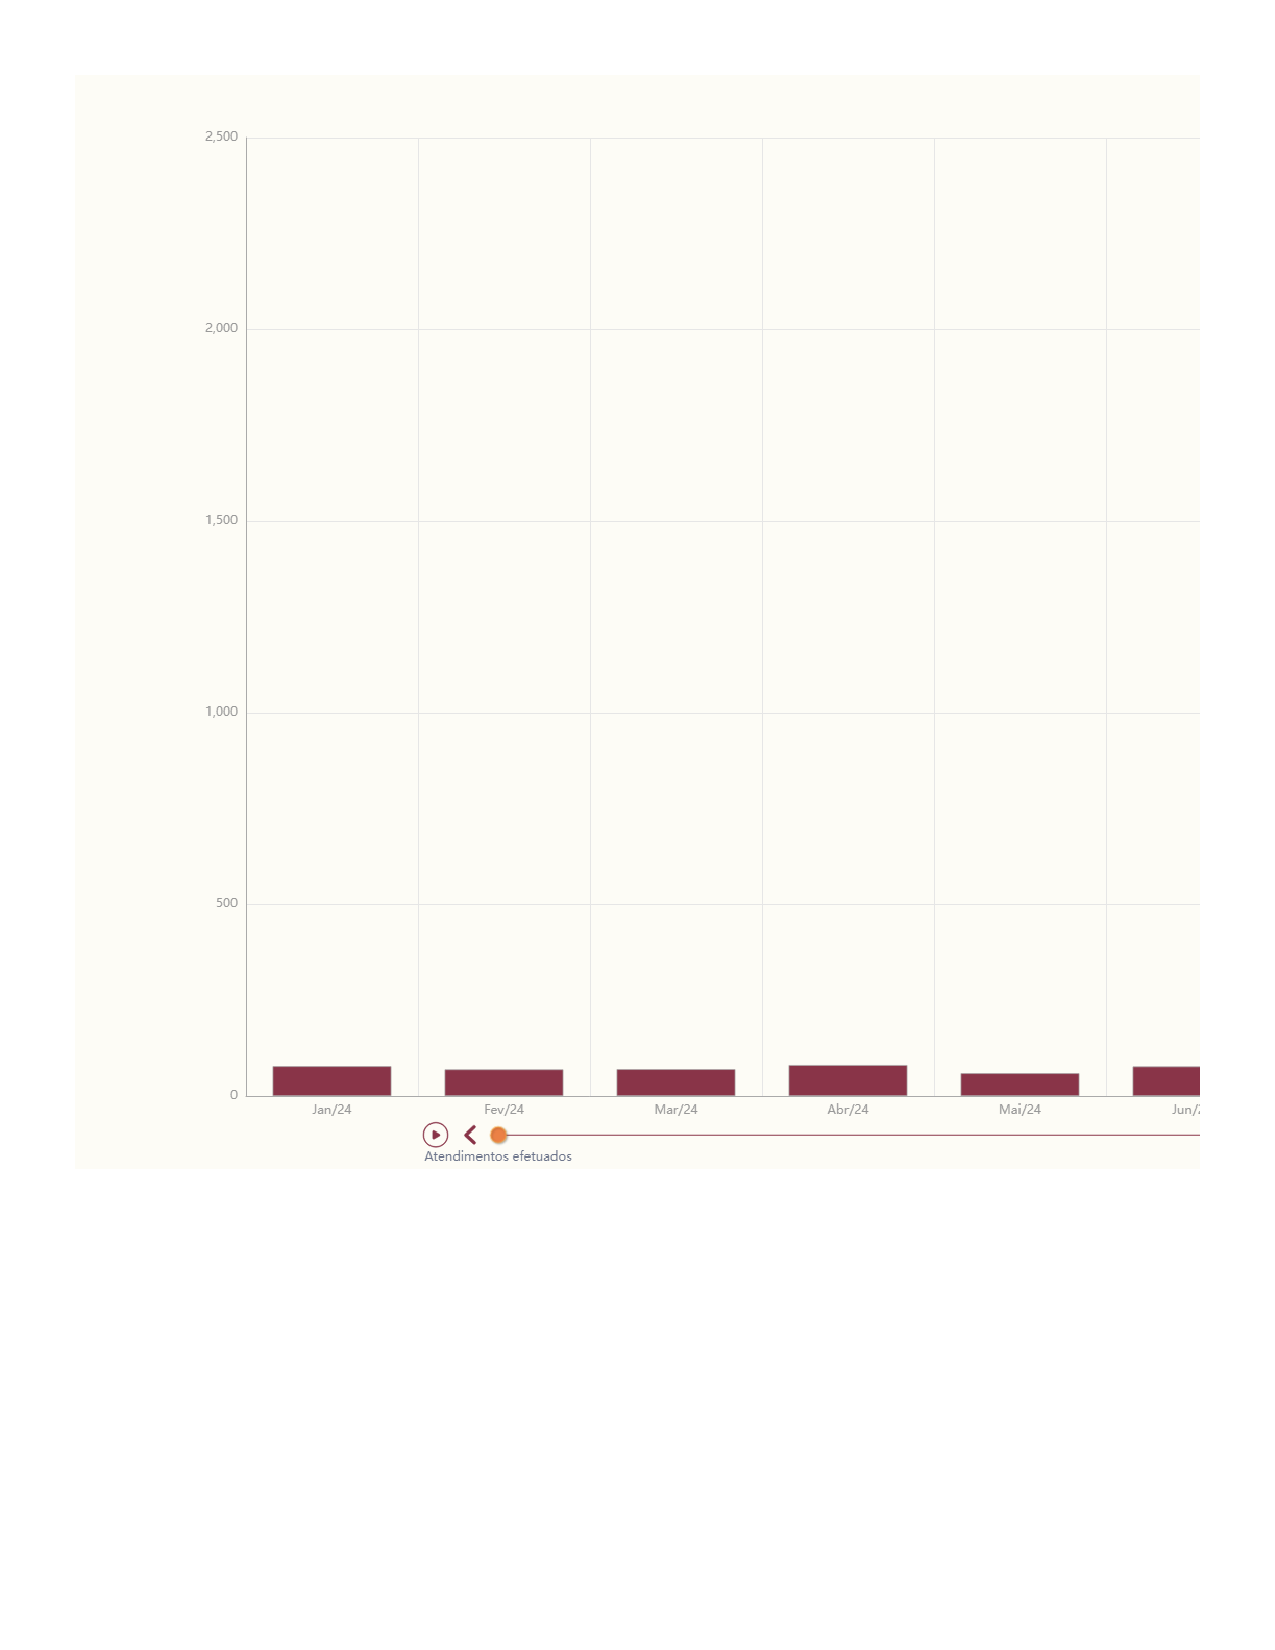
\includegraphics{2024_files/figure-pdf/unnamed-chunk-4-1.pdf}

\section{Parte D}

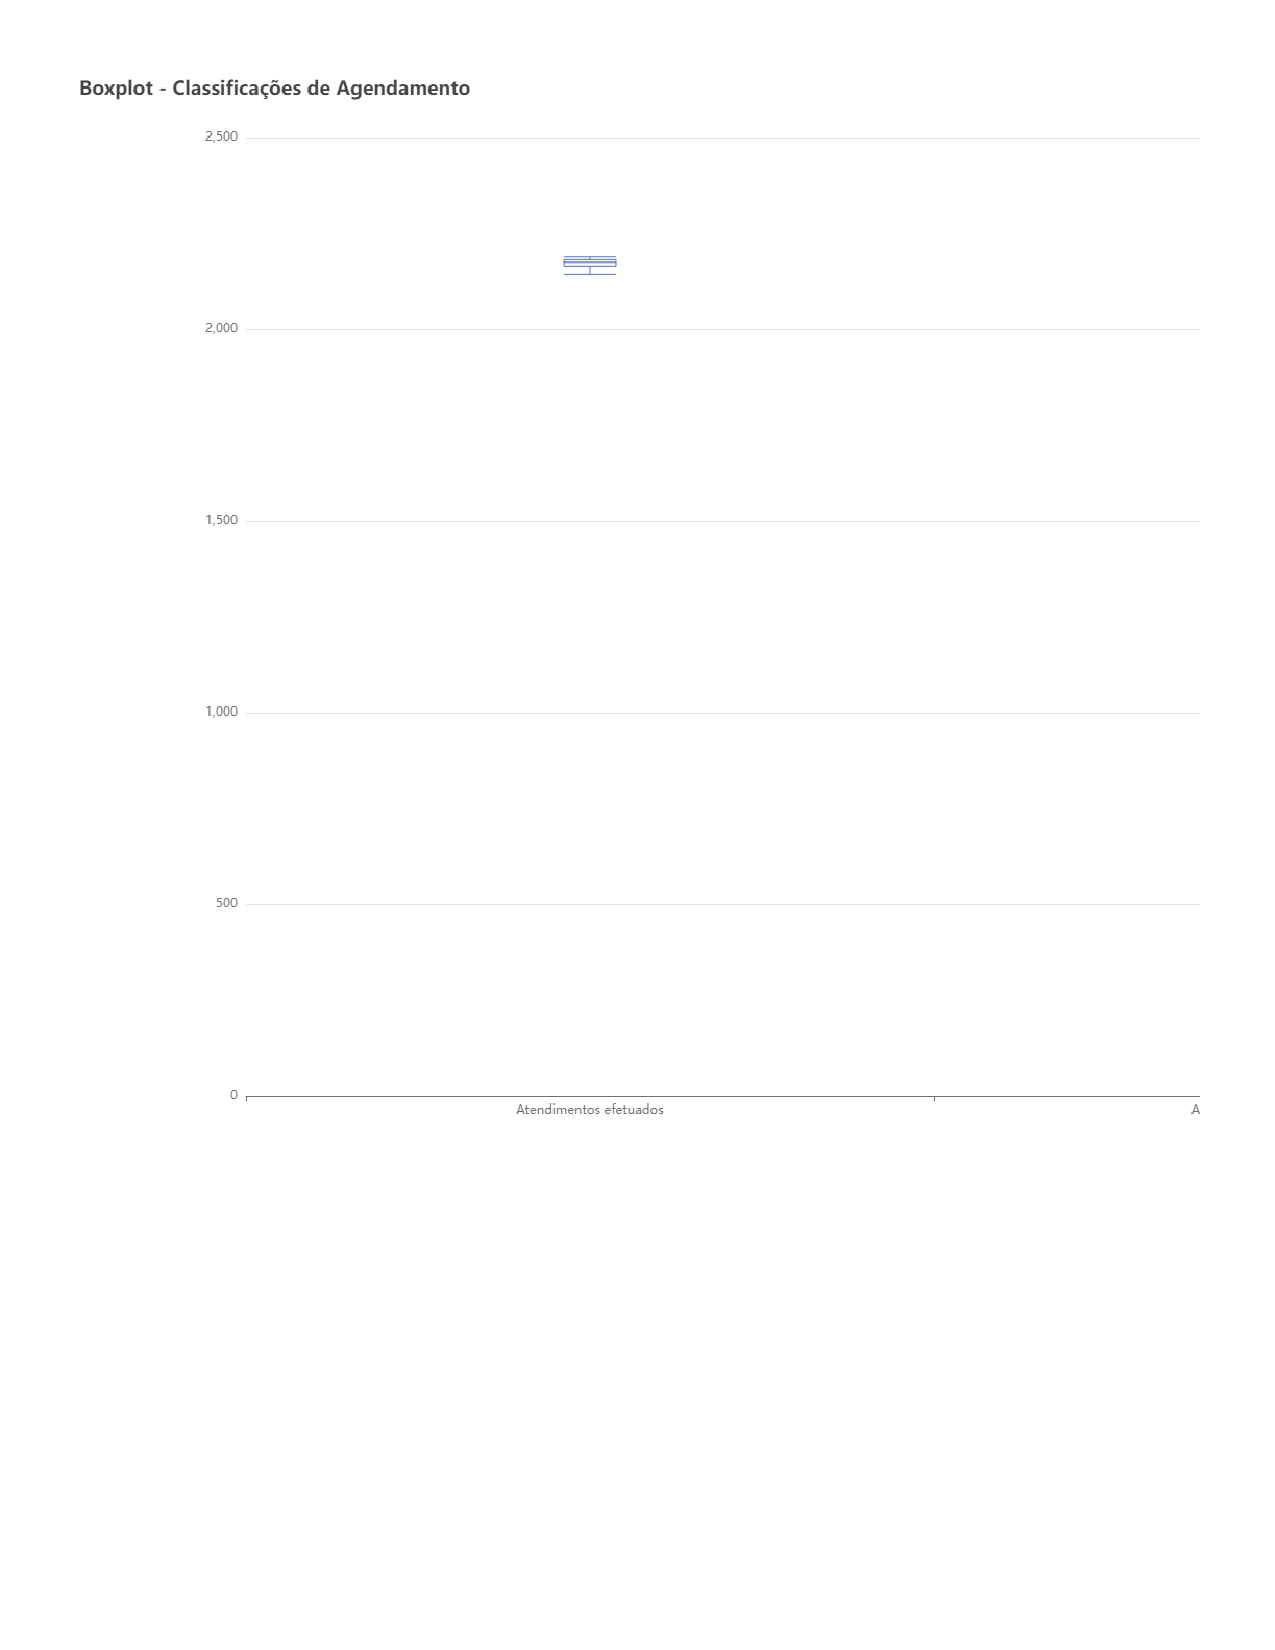
\includegraphics{2024_files/figure-pdf/unnamed-chunk-5-1.pdf}

\hypertarget{atendimentos}{%
\section*{Atendimentos}\label{atendimentos}}
\addcontentsline{toc}{section}{Atendimentos}

\markright{Atendimentos}

\section{Parte A}

\begin{table}
\centering
\caption{Tabela 2.1. Frequência absoluta: Atendimentos.}
\centering
\begin{tabular}[t]{>{}c|>{}c}
\hline
Ano & Frequência Absoluta\\
\hline
\textcolor{black}{\em{\textbf{2024}}} & \textcolor{darkblue}{\textbf{17040}}\\
\hline
\multicolumn{2}{l}{\rule{0pt}{1em}\textit{Fonte: } Tasy.}\\
\end{tabular}
\end{table}

\section{Parte B}

\begin{table}
\centering
\caption{Tabela 2.2. Frequências absoluta e relativa: Classificações de Agendamento  <br><i>Valores agrupados por ano e classificações.</i>}
\centering
\begin{tabular}[t]{>{}c|>{}c|>{}c|>{}c}
\hline
Ano & Classificações de Atendimento & Frequência Absoluta & Frequência relativa (em\%)\\
\hline
\textcolor{black}{\em{\textbf{2024}}} & \textcolor{darkgray}{\em{Interconsulta}} & \textcolor{darkblue}{\textbf{431}} & \textcolor{darkred}{\textbf{2.5}}\\
\hline
\textcolor{black}{\em{\textbf{2024}}} & \textcolor{darkgray}{\em{Primeira Vez}} & \textcolor{darkblue}{\textbf{1457}} & \textcolor{darkred}{\textbf{8.6}}\\
\hline
\textcolor{black}{\em{\textbf{2024}}} & \textcolor{darkgray}{\em{Quimioterapia}} & \textcolor{darkblue}{\textbf{3797}} & \textcolor{darkred}{\textbf{22.3}}\\
\hline
\textcolor{black}{\em{\textbf{2024}}} & \textcolor{darkgray}{\em{Retorno}} & \textcolor{darkblue}{\textbf{11355}} & \textcolor{darkred}{\textbf{66.6}}\\
\hline
\multicolumn{4}{l}{\rule{0pt}{1em}\textit{Fonte: } Tasy.}\\
\end{tabular}
\end{table}

\section{Parte C}

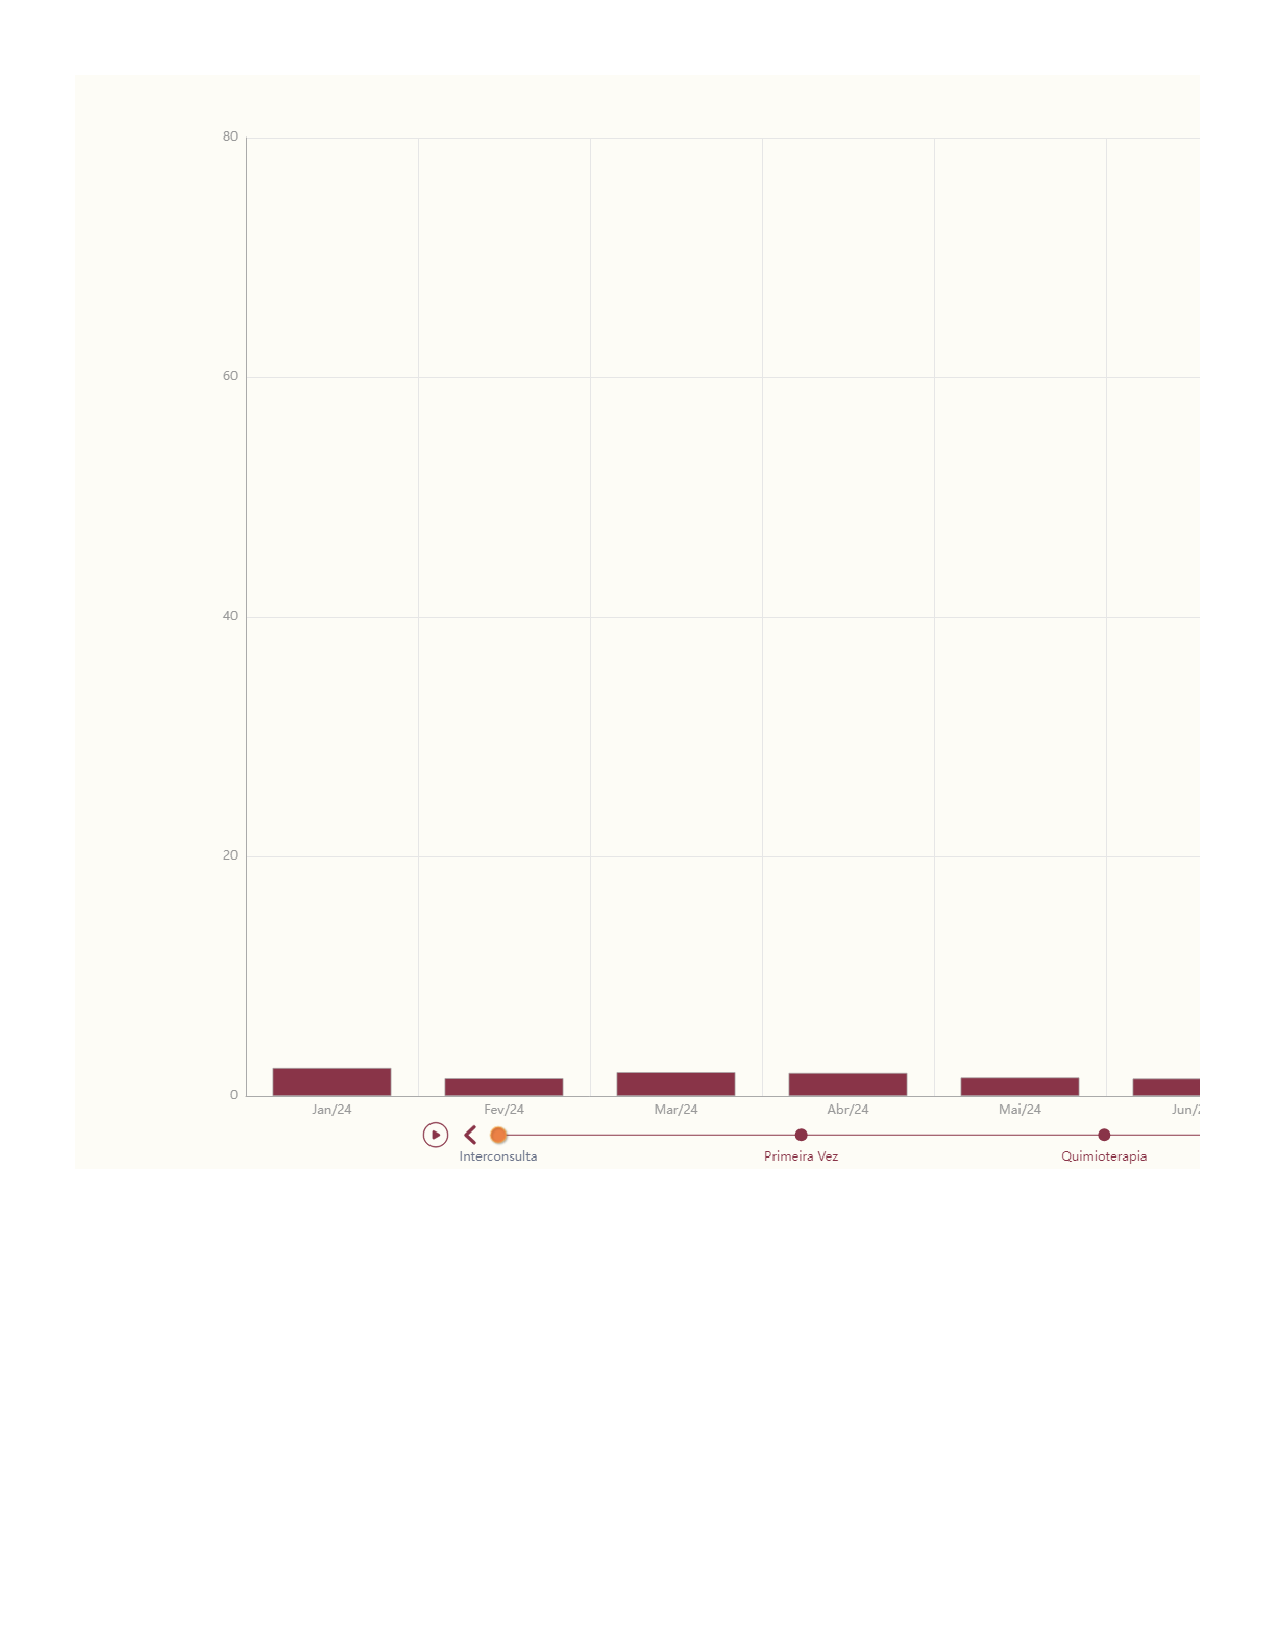
\includegraphics{2024_files/figure-pdf/unnamed-chunk-8-1.pdf}

\section{Parte D}

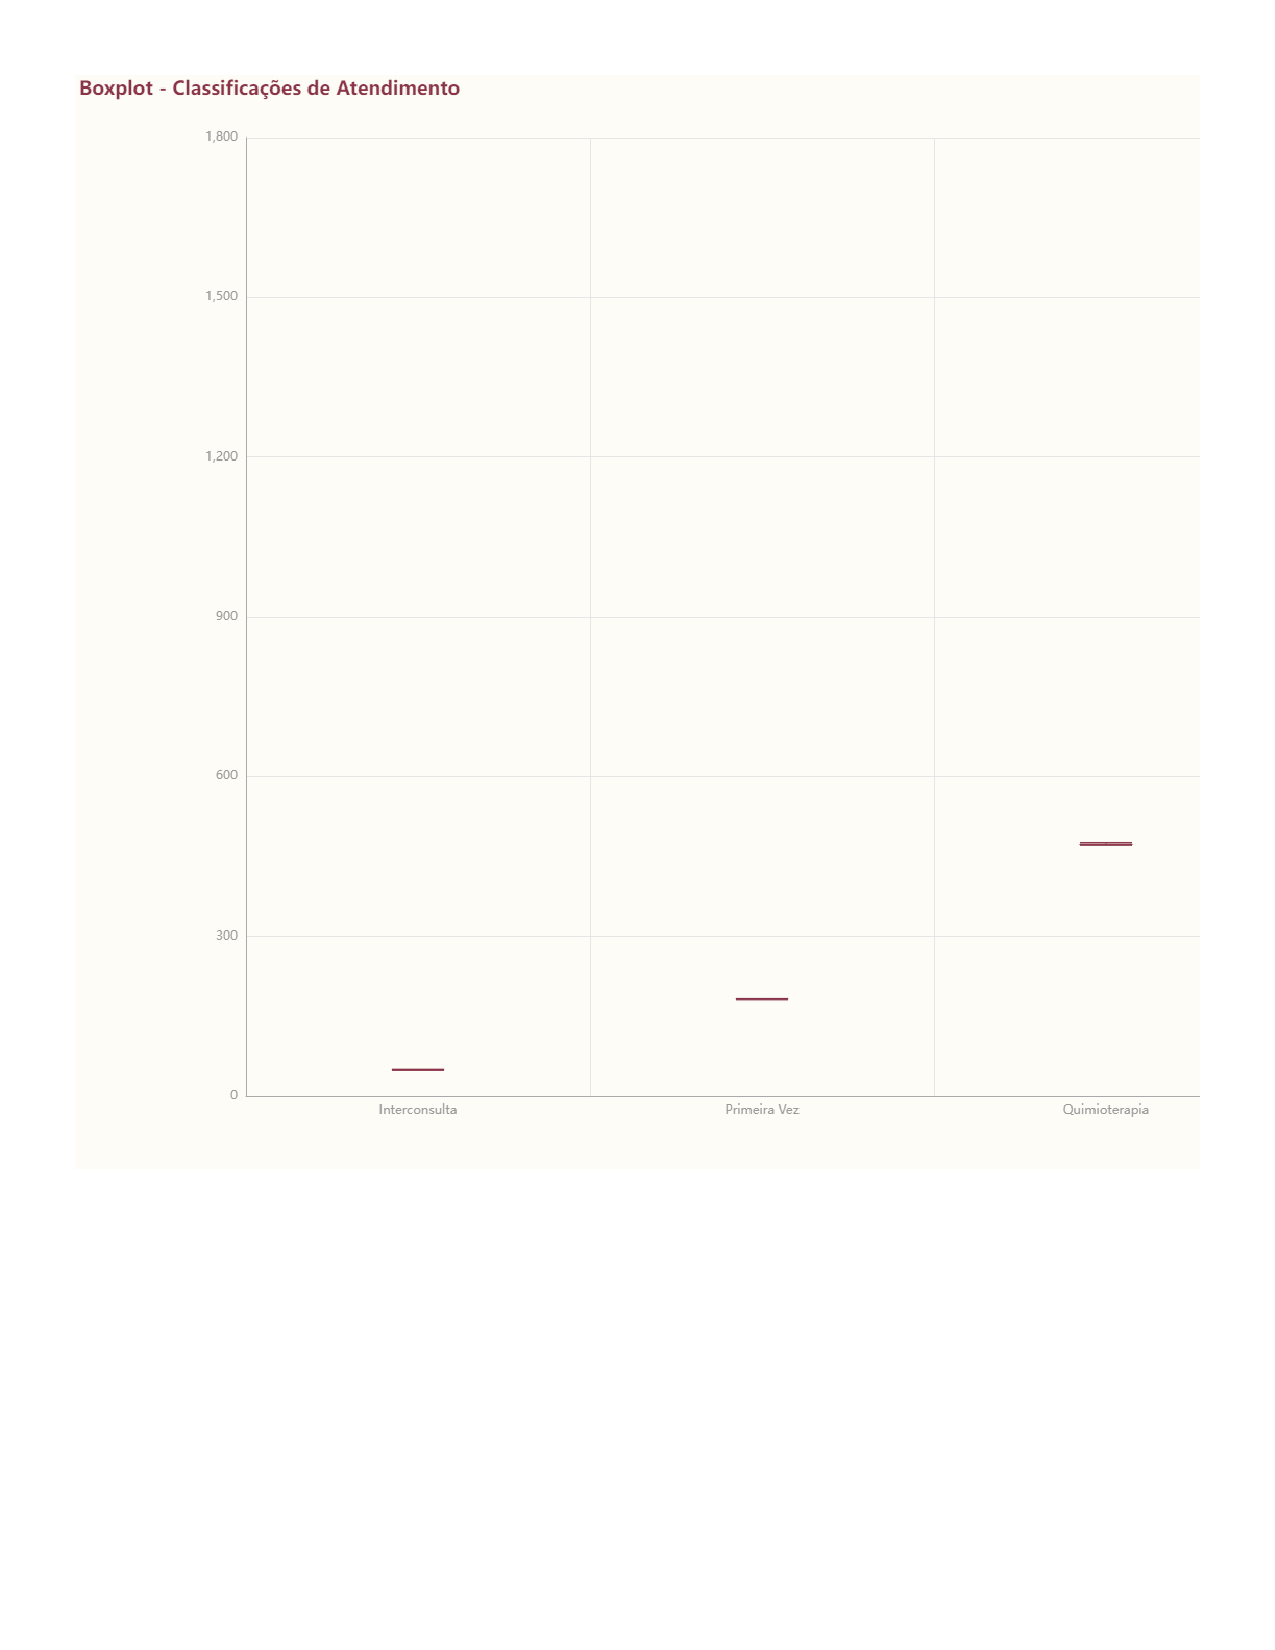
\includegraphics{2024_files/figure-pdf/unnamed-chunk-9-1.pdf}

\part{Parte 02}

\hypertarget{ano-e-peruxedodo-vigentes}{%
\chapter*{Ano e Período vigentes}\label{ano-e-peruxedodo-vigentes}}
\addcontentsline{toc}{chapter}{Ano e Período vigentes}

\markboth{Ano e Período vigentes}{Ano e Período vigentes}

\hypertarget{agendamentos-1}{%
\section*{Agendamentos}\label{agendamentos-1}}
\addcontentsline{toc}{section}{Agendamentos}

\markright{Agendamentos}

\section{Parte A}

\begin{table}
\centering
\caption{Tabela 1.1. Frequências absoluta e relativa: Agendamentos. <br><i>Valores agrupados por ano.</i>}
\centering
\begin{tabular}[t]{>{}c|>{}c|>{}c}
\hline
Ano & Frequência Absoluta & Frequência relativa (em\%)\\
\hline
\textcolor{black}{\em{\textbf{2022}}} & \textcolor{darkblue}{\textbf{18207}} & \textcolor{darkred}{\textbf{33.2}}\\
\hline
\textcolor{black}{\em{\textbf{2023}}} & \textcolor{darkblue}{\textbf{18736}} & \textcolor{darkred}{\textbf{34.1}}\\
\hline
\textcolor{black}{\em{\textbf{2024}}} & \textcolor{darkblue}{\textbf{17941}} & \textcolor{darkred}{\textbf{32.7}}\\
\hline
\multicolumn{3}{l}{\rule{0pt}{1em}\textit{Fonte: } Tasy.}\\
\end{tabular}
\end{table}

\section{Parte B}

\begin{table}
\centering
\caption{Tabela 1.2. Frequências absoluta e relativa: Classificações de Agendamento  <br><i>Valores agrupados por ano e classificações.</i>}
\centering
\begin{tabular}[t]{>{}c|>{}c|>{}c|>{}c}
\hline
Ano & Classificações de Agendamento & Frequência Absoluta & Frequência relativa (em\%)\\
\hline
\textcolor{black}{\em{\textbf{2022}}} & \textcolor{darkgray}{\em{Atendimentos efetuados}} & \textcolor{darkblue}{\textbf{16461}} & \textcolor{darkred}{\textbf{90.4}}\\
\hline
\textcolor{black}{\em{\textbf{2022}}} & \textcolor{darkgray}{\em{Atendimentos não efetuados}} & \textcolor{darkblue}{\textbf{1746}} & \textcolor{darkred}{\textbf{9.6}}\\
\hline
\textcolor{black}{\em{\textbf{2023}}} & \textcolor{darkgray}{\em{Atendimentos efetuados}} & \textcolor{darkblue}{\textbf{17229}} & \textcolor{darkred}{\textbf{92.0}}\\
\hline
\textcolor{black}{\em{\textbf{2023}}} & \textcolor{darkgray}{\em{Atendimentos não efetuados}} & \textcolor{darkblue}{\textbf{1507}} & \textcolor{darkred}{\textbf{8.0}}\\
\hline
\textcolor{black}{\em{\textbf{2024}}} & \textcolor{darkgray}{\em{Atendimentos efetuados}} & \textcolor{darkblue}{\textbf{17040}} & \textcolor{darkred}{\textbf{95.0}}\\
\hline
\textcolor{black}{\em{\textbf{2024}}} & \textcolor{darkgray}{\em{Atendimentos não efetuados}} & \textcolor{darkblue}{\textbf{901}} & \textcolor{darkred}{\textbf{5.0}}\\
\hline
\multicolumn{4}{l}{\rule{0pt}{1em}\textit{Fonte: } Tasy.}\\
\end{tabular}
\end{table}

\section{Parte C}

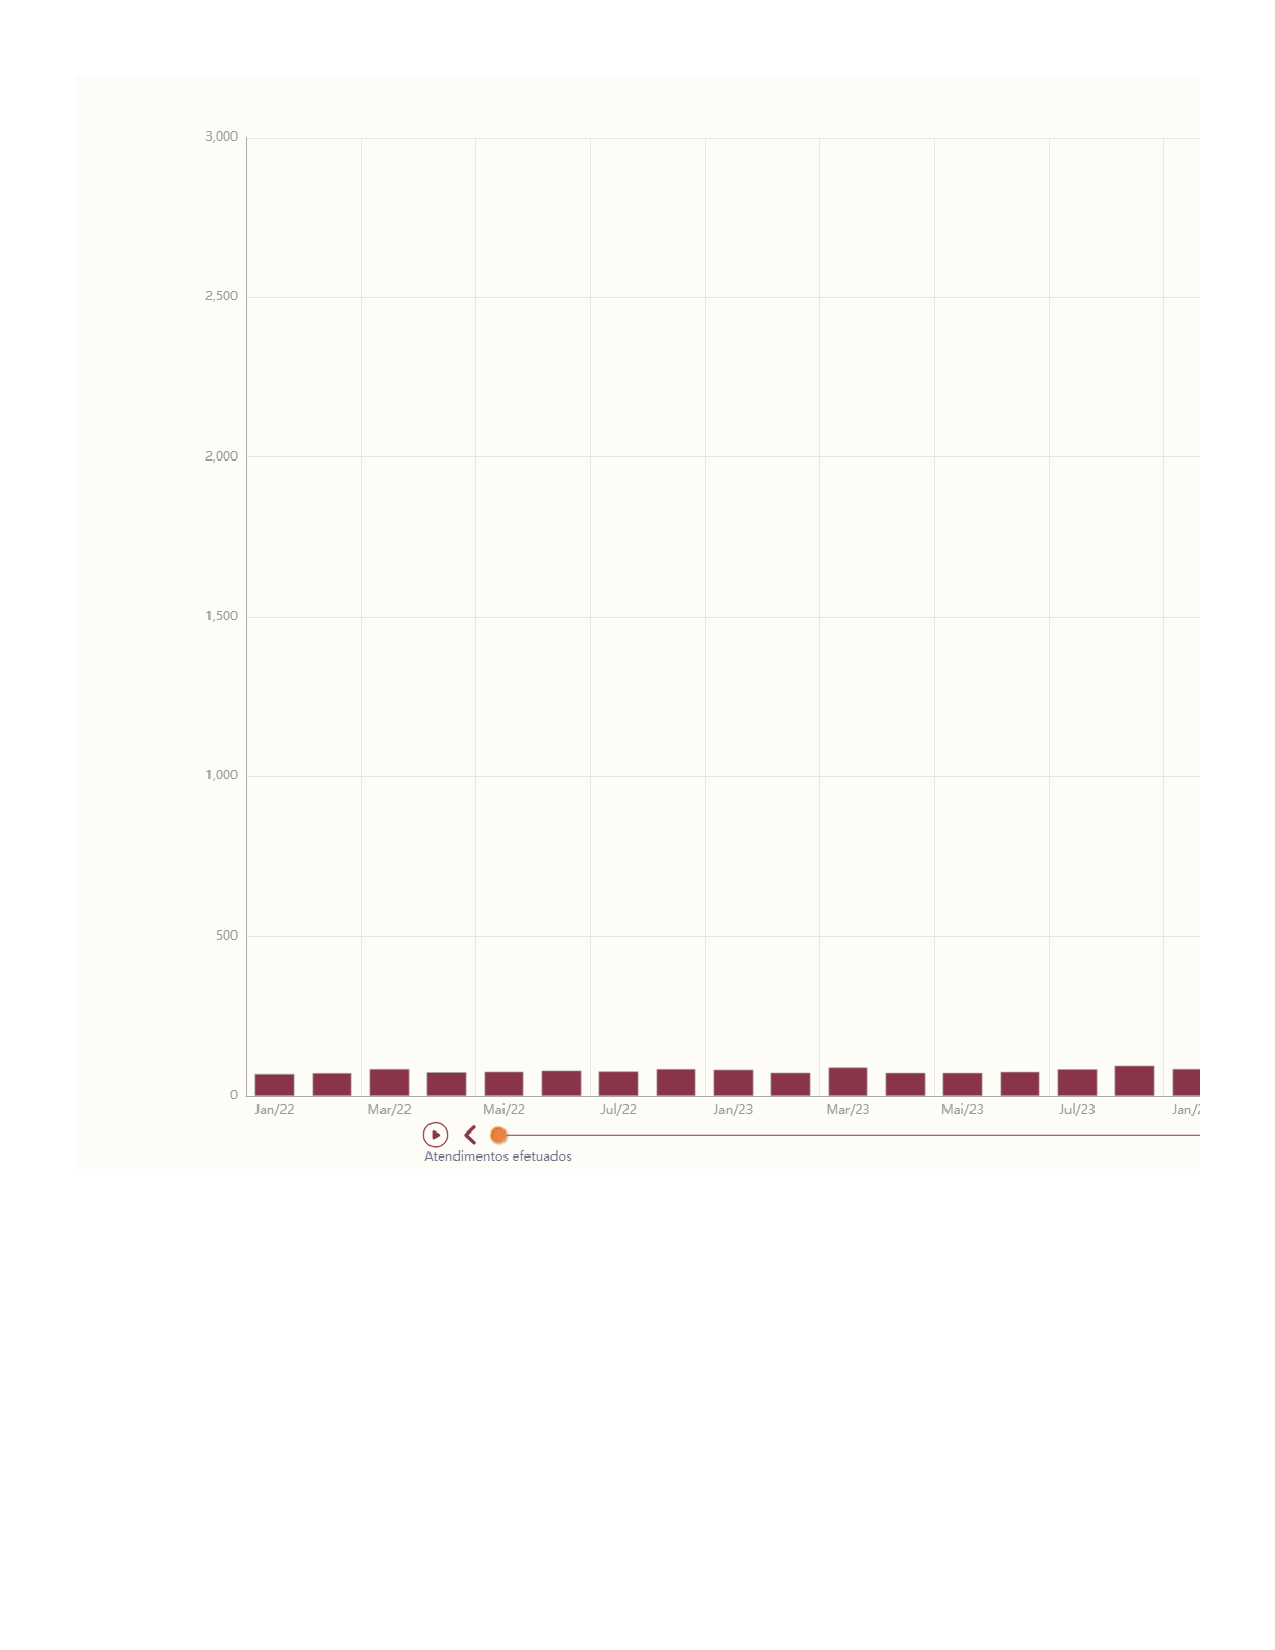
\includegraphics{intro_files/figure-pdf/unnamed-chunk-4-1.pdf}

\section{Parte D}

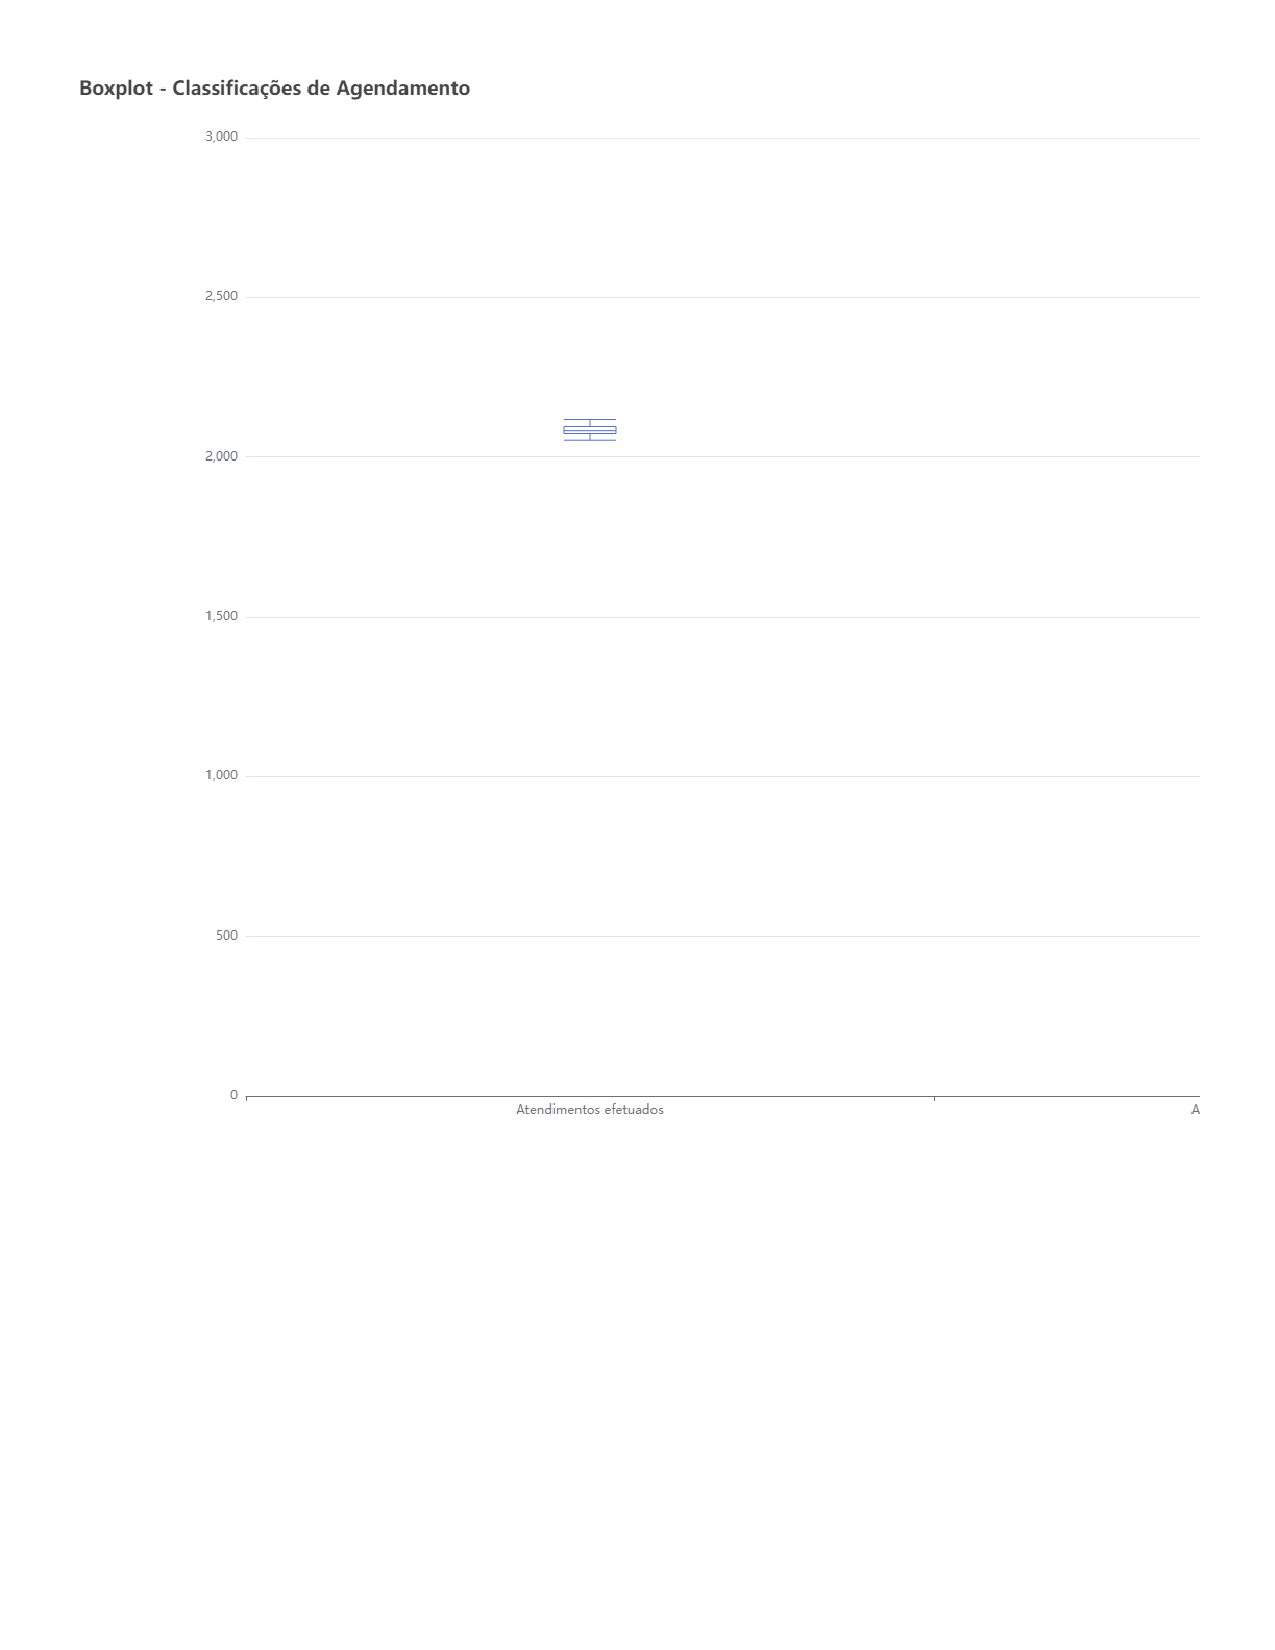
\includegraphics{intro_files/figure-pdf/unnamed-chunk-5-1.pdf}

\hypertarget{atendimentos-1}{%
\section*{Atendimentos}\label{atendimentos-1}}
\addcontentsline{toc}{section}{Atendimentos}

\markright{Atendimentos}

\section{Parte A}

\begin{table}
\centering
\caption{Tabela 2.1. Frequências absoluta e relativa: Agendamentos. <br><i>Valores agrupados por ano.</i>}
\centering
\begin{tabular}[t]{>{}c|>{}c|>{}c}
\hline
Ano & Frequência Absoluta & Frequência relativa (em\%)\\
\hline
\textcolor{black}{\em{\textbf{2022}}} & \textcolor{darkblue}{\textbf{16461}} & \textcolor{darkred}{\textbf{32.4}}\\
\hline
\textcolor{black}{\em{\textbf{2023}}} & \textcolor{darkblue}{\textbf{17229}} & \textcolor{darkred}{\textbf{34.0}}\\
\hline
\textcolor{black}{\em{\textbf{2024}}} & \textcolor{darkblue}{\textbf{17040}} & \textcolor{darkred}{\textbf{33.6}}\\
\hline
\multicolumn{3}{l}{\rule{0pt}{1em}\textit{Fonte: } Tasy.}\\
\end{tabular}
\end{table}

\section{Parte B}

\begin{table}
\centering
\caption{Tabela 2.2. Frequências absoluta e relativa: Classificações de Agendamento  <br><i>Valores agrupados por ano e classificações.</i>}
\centering
\begin{tabular}[t]{>{}c|>{}c|>{}c|>{}c}
\hline
Ano & Classificações de Atendimento & Frequência Absoluta & Frequência relativa (em\%)\\
\hline
\textcolor{black}{\em{\textbf{2022}}} & \textcolor{darkgray}{\em{Interconsulta}} & \textcolor{darkblue}{\textbf{303}} & \textcolor{darkred}{\textbf{1.8}}\\
\hline
\textcolor{black}{\em{\textbf{2022}}} & \textcolor{darkgray}{\em{Primeira Vez}} & \textcolor{darkblue}{\textbf{1577}} & \textcolor{darkred}{\textbf{9.6}}\\
\hline
\textcolor{black}{\em{\textbf{2022}}} & \textcolor{darkgray}{\em{Quimioterapia}} & \textcolor{darkblue}{\textbf{2180}} & \textcolor{darkred}{\textbf{13.2}}\\
\hline
\textcolor{black}{\em{\textbf{2022}}} & \textcolor{darkgray}{\em{Retorno}} & \textcolor{darkblue}{\textbf{12401}} & \textcolor{darkred}{\textbf{75.3}}\\
\hline
\textcolor{black}{\em{\textbf{2023}}} & \textcolor{darkgray}{\em{Interconsulta}} & \textcolor{darkblue}{\textbf{272}} & \textcolor{darkred}{\textbf{1.6}}\\
\hline
\textcolor{black}{\em{\textbf{2023}}} & \textcolor{darkgray}{\em{Primeira Vez}} & \textcolor{darkblue}{\textbf{1551}} & \textcolor{darkred}{\textbf{9.0}}\\
\hline
\textcolor{black}{\em{\textbf{2023}}} & \textcolor{darkgray}{\em{Quimioterapia}} & \textcolor{darkblue}{\textbf{3201}} & \textcolor{darkred}{\textbf{18.6}}\\
\hline
\textcolor{black}{\em{\textbf{2023}}} & \textcolor{darkgray}{\em{Retorno}} & \textcolor{darkblue}{\textbf{12205}} & \textcolor{darkred}{\textbf{70.8}}\\
\hline
\textcolor{black}{\em{\textbf{2024}}} & \textcolor{darkgray}{\em{Interconsulta}} & \textcolor{darkblue}{\textbf{431}} & \textcolor{darkred}{\textbf{2.5}}\\
\hline
\textcolor{black}{\em{\textbf{2024}}} & \textcolor{darkgray}{\em{Primeira Vez}} & \textcolor{darkblue}{\textbf{1457}} & \textcolor{darkred}{\textbf{8.6}}\\
\hline
\textcolor{black}{\em{\textbf{2024}}} & \textcolor{darkgray}{\em{Quimioterapia}} & \textcolor{darkblue}{\textbf{3797}} & \textcolor{darkred}{\textbf{22.3}}\\
\hline
\textcolor{black}{\em{\textbf{2024}}} & \textcolor{darkgray}{\em{Retorno}} & \textcolor{darkblue}{\textbf{11355}} & \textcolor{darkred}{\textbf{66.6}}\\
\hline
\multicolumn{4}{l}{\rule{0pt}{1em}\textit{Fonte: } Tasy.}\\
\end{tabular}
\end{table}

\section{Parte C}

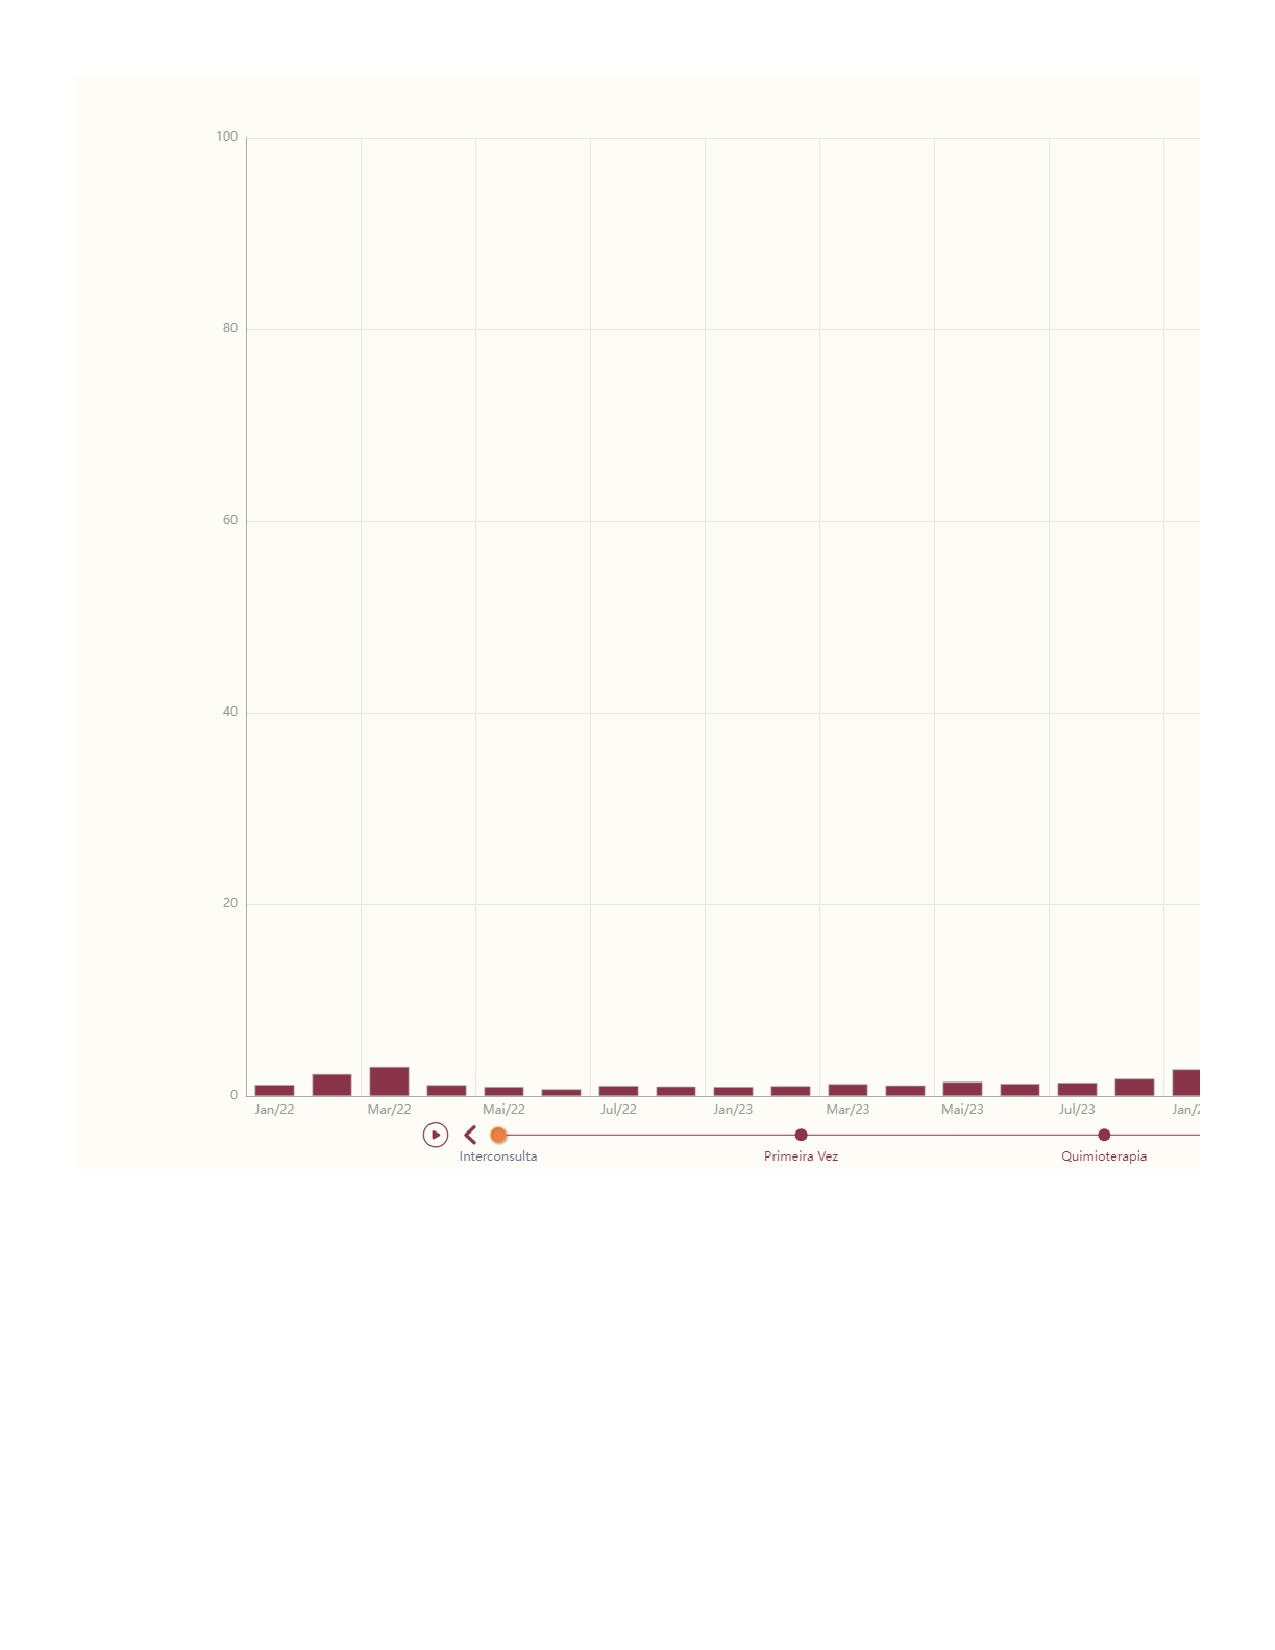
\includegraphics{intro_files/figure-pdf/unnamed-chunk-8-1.pdf}

\section{Parte D}

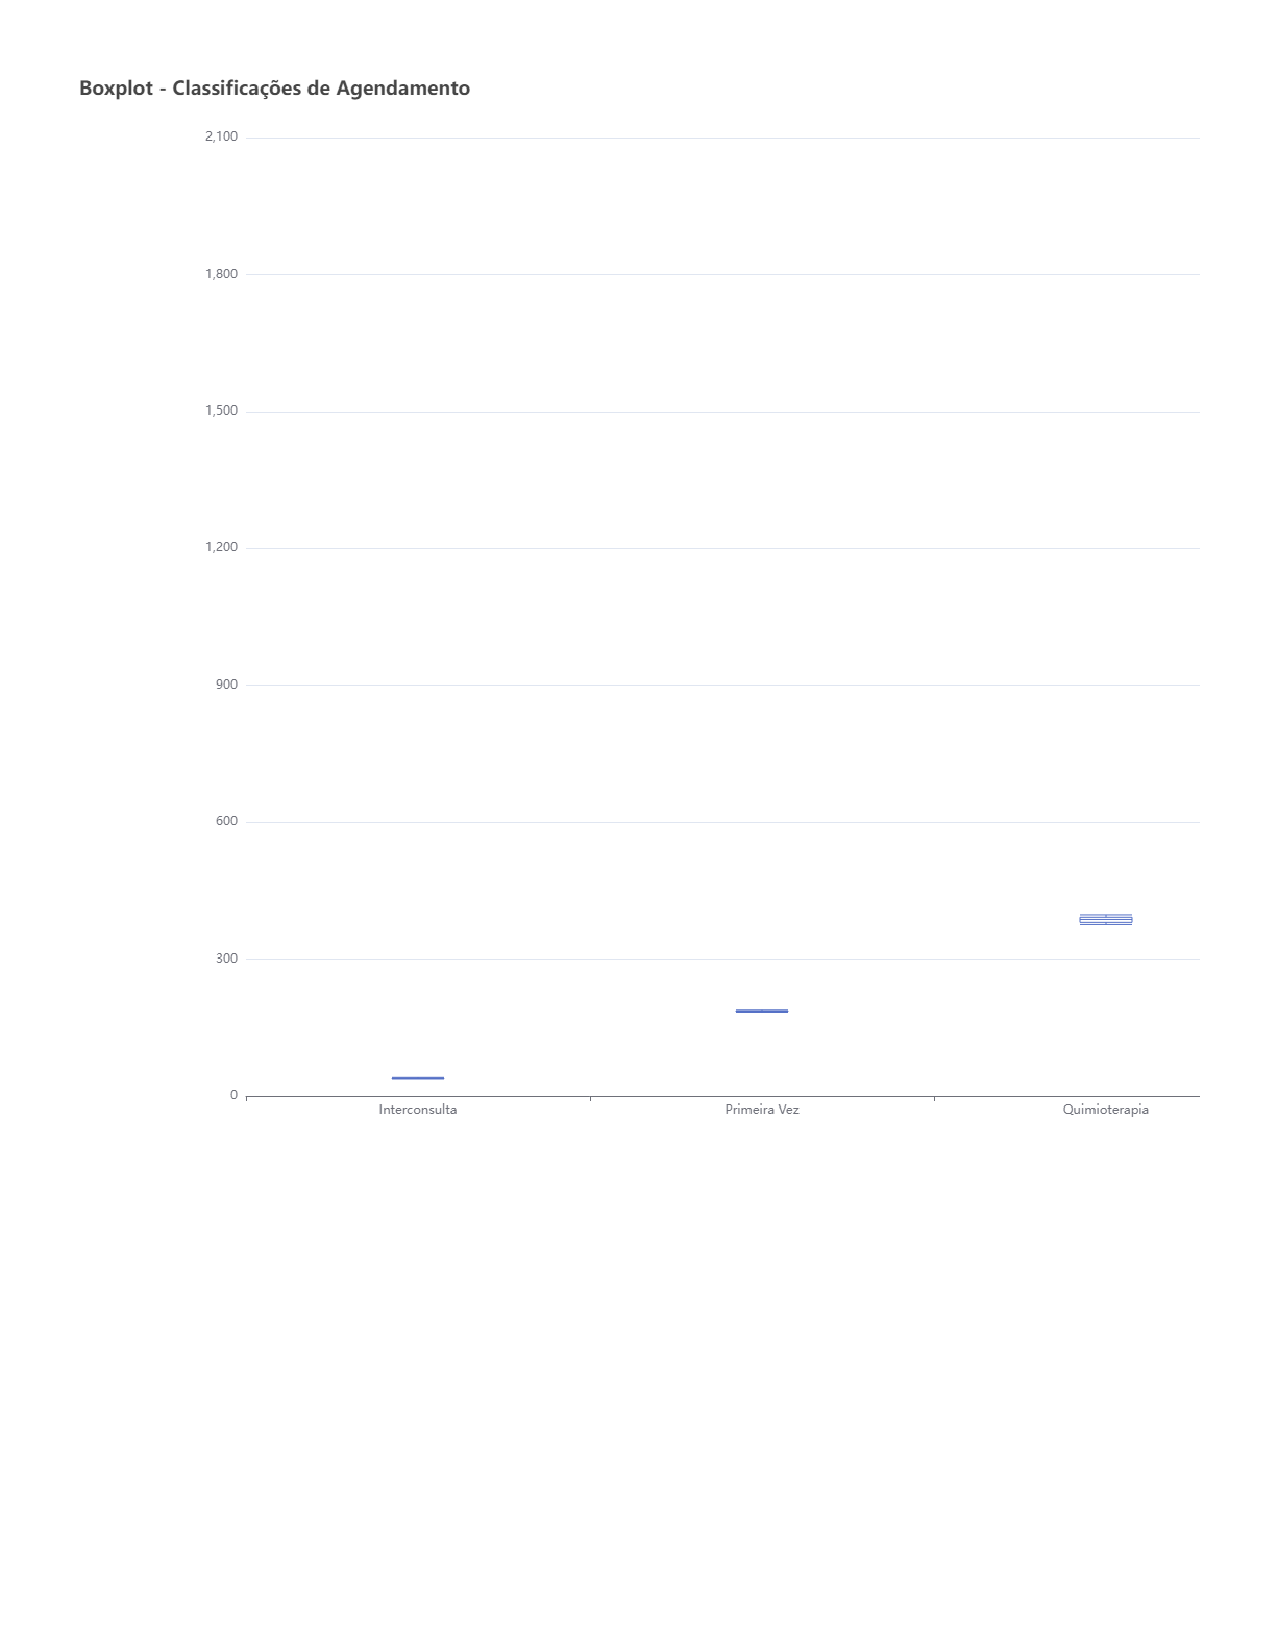
\includegraphics{intro_files/figure-pdf/unnamed-chunk-9-1.pdf}

\part{Parte 03}

\hypertarget{ano-2023-peruxedodo-janeiro---dezembro}{%
\chapter*{Ano: 2023 \textbar{} Período: Janeiro -
Dezembro}\label{ano-2023-peruxedodo-janeiro---dezembro}}
\addcontentsline{toc}{chapter}{Ano: 2023 \textbar{} Período: Janeiro -
Dezembro}

\markboth{Ano: 2023 \textbar{} Período: Janeiro - Dezembro}{Ano: 2023
\textbar{} Período: Janeiro - Dezembro}

\hypertarget{agendamentos-2}{%
\section*{Agendamentos}\label{agendamentos-2}}
\addcontentsline{toc}{section}{Agendamentos}

\markright{Agendamentos}

\section{Parte A}

\begin{table}
\centering
\caption{Tabela 3.1. Frequência absoluta: Agendamentos.}
\centering
\begin{tabular}[t]{>{}c|>{}c}
\hline
Ano & Frequência Absoluta\\
\hline
\textcolor{black}{\em{\textbf{2023}}} & \textcolor{darkblue}{\textbf{27063}}\\
\hline
\multicolumn{2}{l}{\rule{0pt}{1em}\textit{Fonte: } Tasy.}\\
\end{tabular}
\end{table}

\section{Parte B}

\begin{table}
\centering
\caption{Tabela 3.2. Frequências absoluta e relativa: Classificações de Agendamento  <br><i>Valores agrupados por ano e classificações.</i>}
\centering
\begin{tabular}[t]{>{}c|>{}c|>{}c|>{}c}
\hline
Ano & Classificações de Agendamento & Frequência Absoluta & Frequência relativa (em\%)\\
\hline
\textcolor{black}{\em{\textbf{2023}}} & \textcolor{darkgray}{\em{Atendimentos efetuados}} & \textcolor{darkblue}{\textbf{24924}} & \textcolor{darkred}{\textbf{92.1}}\\
\hline
\textcolor{black}{\em{\textbf{2023}}} & \textcolor{darkgray}{\em{Atendimentos não efetuados}} & \textcolor{darkblue}{\textbf{2139}} & \textcolor{darkred}{\textbf{7.9}}\\
\hline
\multicolumn{4}{l}{\rule{0pt}{1em}\textit{Fonte: } Tasy.}\\
\end{tabular}
\end{table}

\section{Parte C}

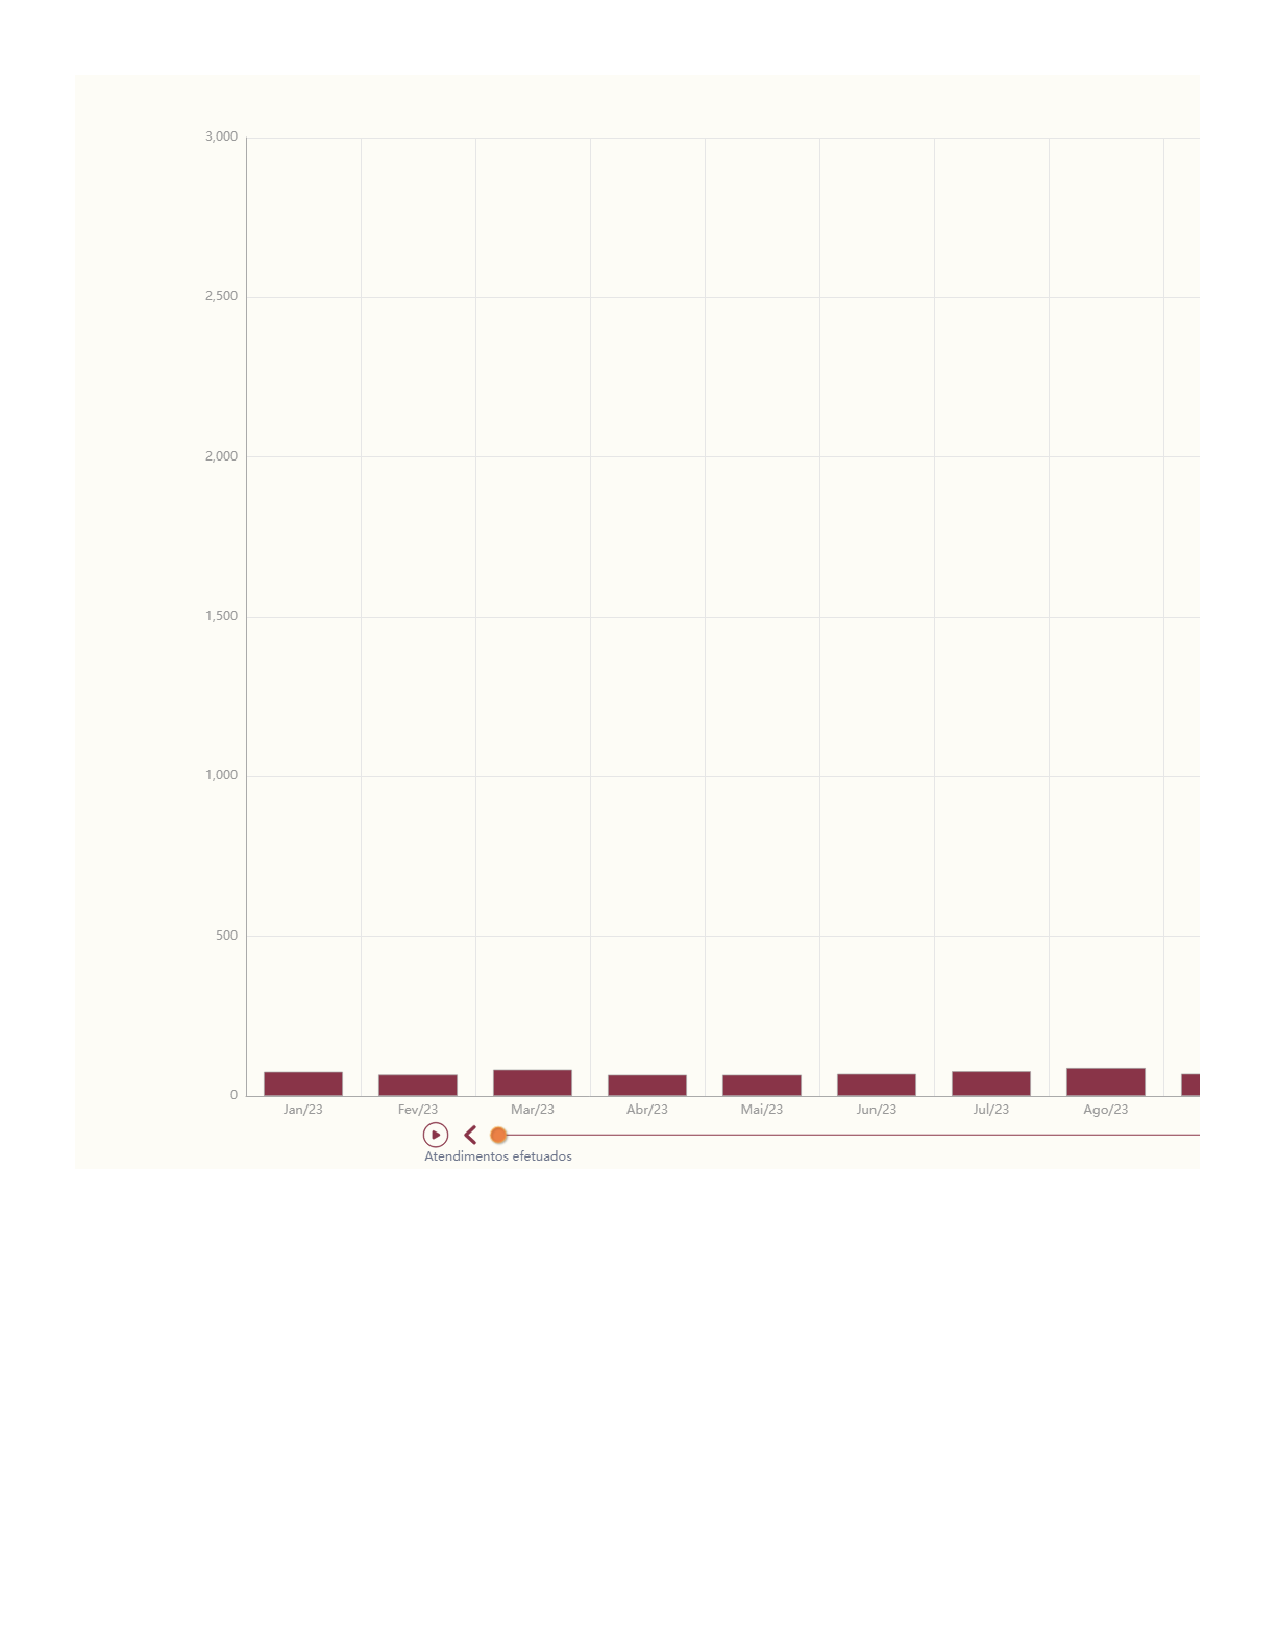
\includegraphics{2023_files/figure-pdf/unnamed-chunk-4-1.pdf}

\section{Parte D}

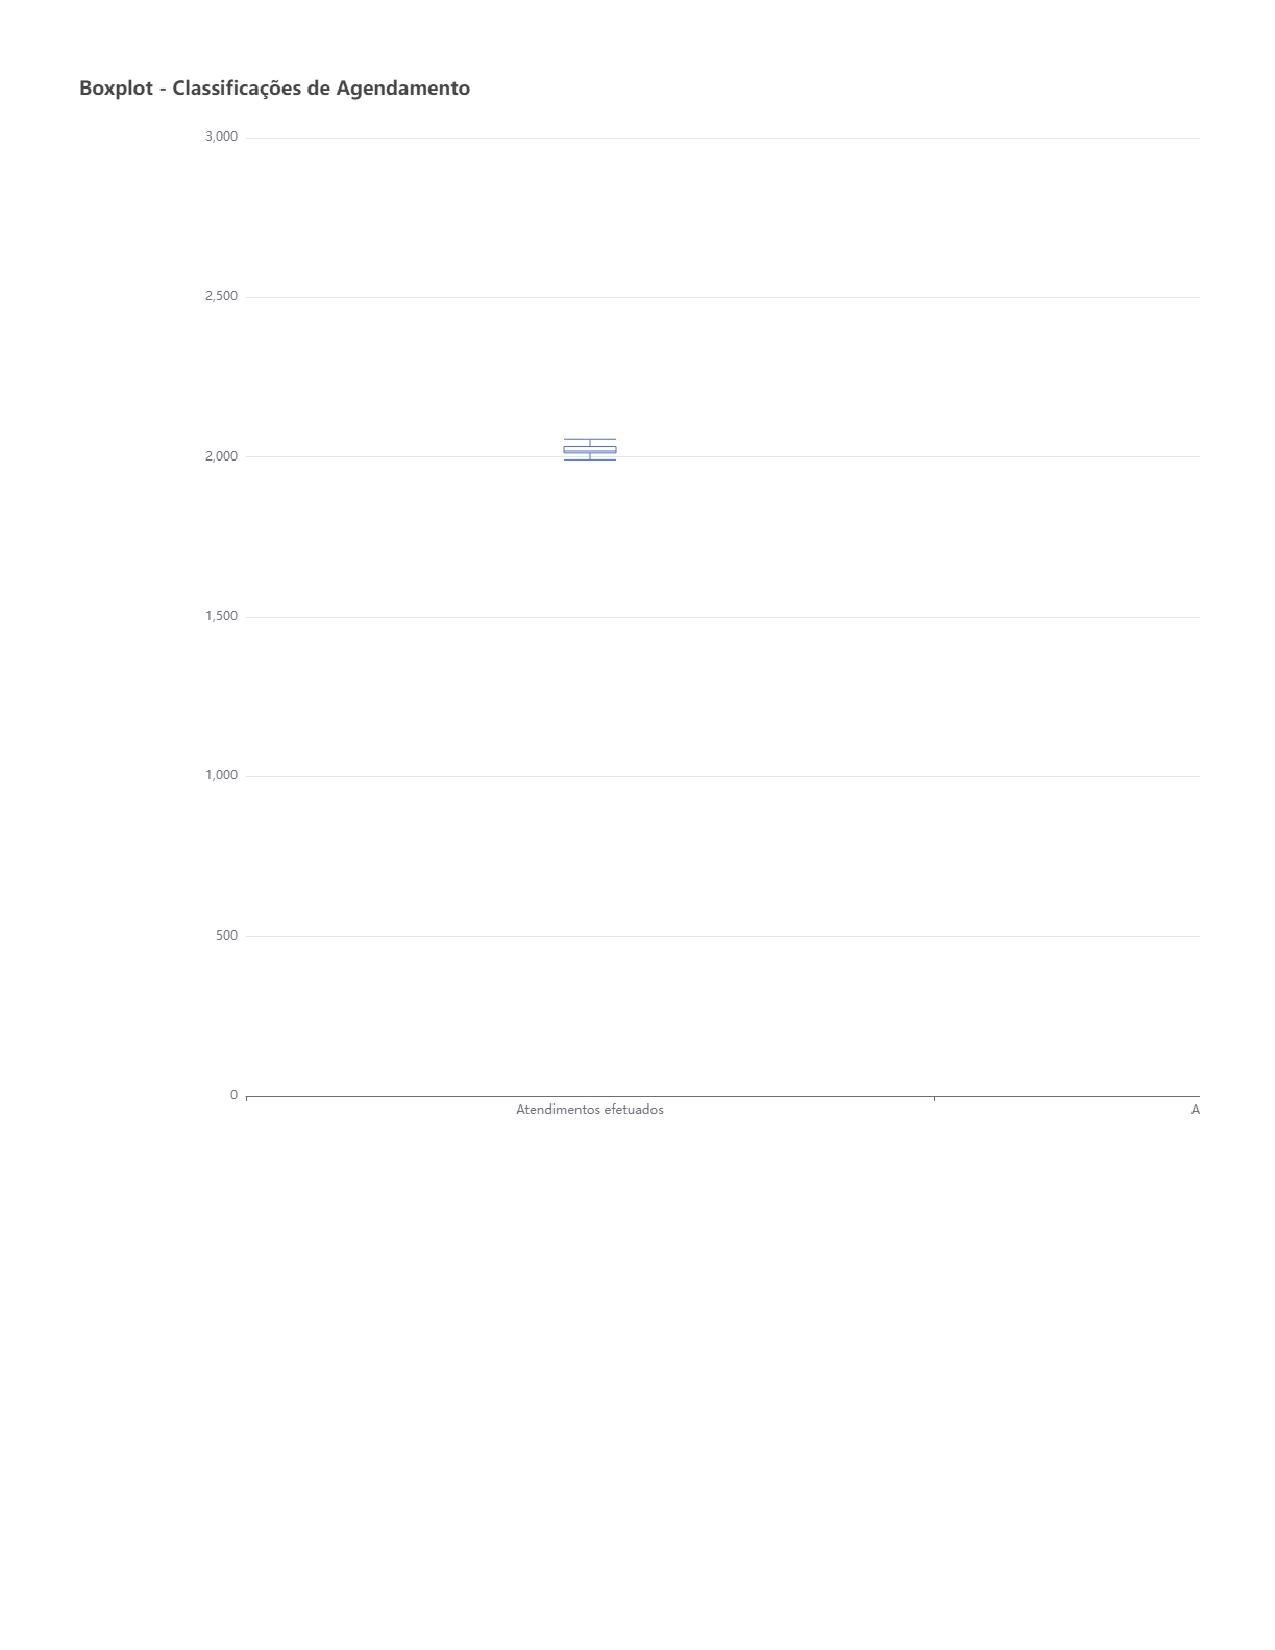
\includegraphics{2023_files/figure-pdf/unnamed-chunk-5-1.pdf}

\hypertarget{atendimentos-2}{%
\section*{Atendimentos}\label{atendimentos-2}}
\addcontentsline{toc}{section}{Atendimentos}

\markright{Atendimentos}

\section{Parte A}

\begin{table}
\centering
\caption{Tabela 2.1. Frequência absoluta: Atendimentos.}
\centering
\begin{tabular}[t]{>{}c|>{}c}
\hline
Ano & Frequência Absoluta\\
\hline
\textcolor{black}{\em{\textbf{2023}}} & \textcolor{darkblue}{\textbf{24924}}\\
\hline
\multicolumn{2}{l}{\rule{0pt}{1em}\textit{Fonte: } Tasy.}\\
\end{tabular}
\end{table}

\section{Parte B}

\begin{table}
\centering
\caption{Tabela 2.2. Frequências absoluta e relativa: Classificações de Agendamento  <br><i>Valores agrupados por ano e classificações.</i>}
\centering
\begin{tabular}[t]{>{}c|>{}c|>{}c|>{}c}
\hline
Ano & Classificações de Atendimento & Frequência Absoluta & Frequência relativa (em\%)\\
\hline
\textcolor{black}{\em{\textbf{2023}}} & \textcolor{darkgray}{\em{Interconsulta}} & \textcolor{darkblue}{\textbf{509}} & \textcolor{darkred}{\textbf{2}}\\
\hline
\textcolor{black}{\em{\textbf{2023}}} & \textcolor{darkgray}{\em{Primeira Vez}} & \textcolor{darkblue}{\textbf{1991}} & \textcolor{darkred}{\textbf{8}}\\
\hline
\textcolor{black}{\em{\textbf{2023}}} & \textcolor{darkgray}{\em{Quimioterapia}} & \textcolor{darkblue}{\textbf{4733}} & \textcolor{darkred}{\textbf{19}}\\
\hline
\textcolor{black}{\em{\textbf{2023}}} & \textcolor{darkgray}{\em{Retorno}} & \textcolor{darkblue}{\textbf{17691}} & \textcolor{darkred}{\textbf{71}}\\
\hline
\multicolumn{4}{l}{\rule{0pt}{1em}\textit{Fonte: } Tasy.}\\
\end{tabular}
\end{table}

\section{Parte C}

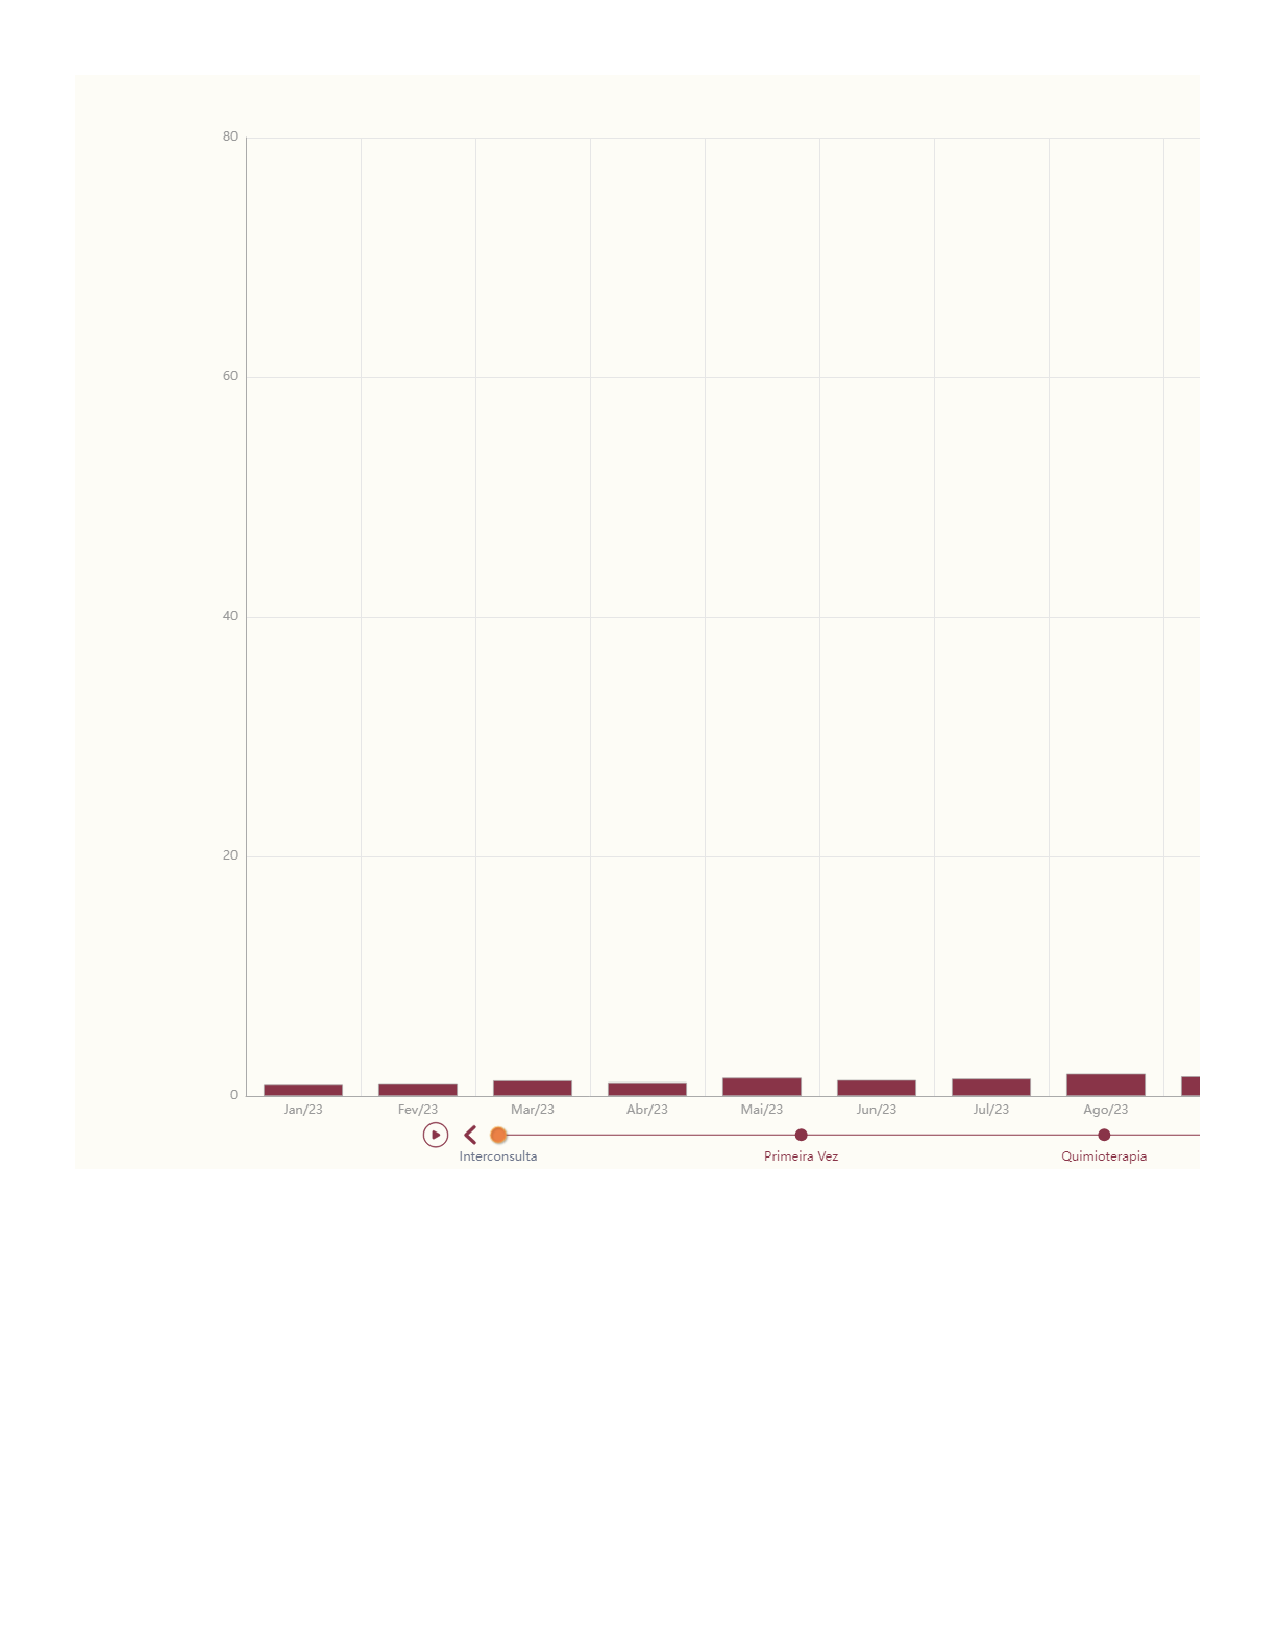
\includegraphics{2023_files/figure-pdf/unnamed-chunk-8-1.pdf}

\section{Parte D}

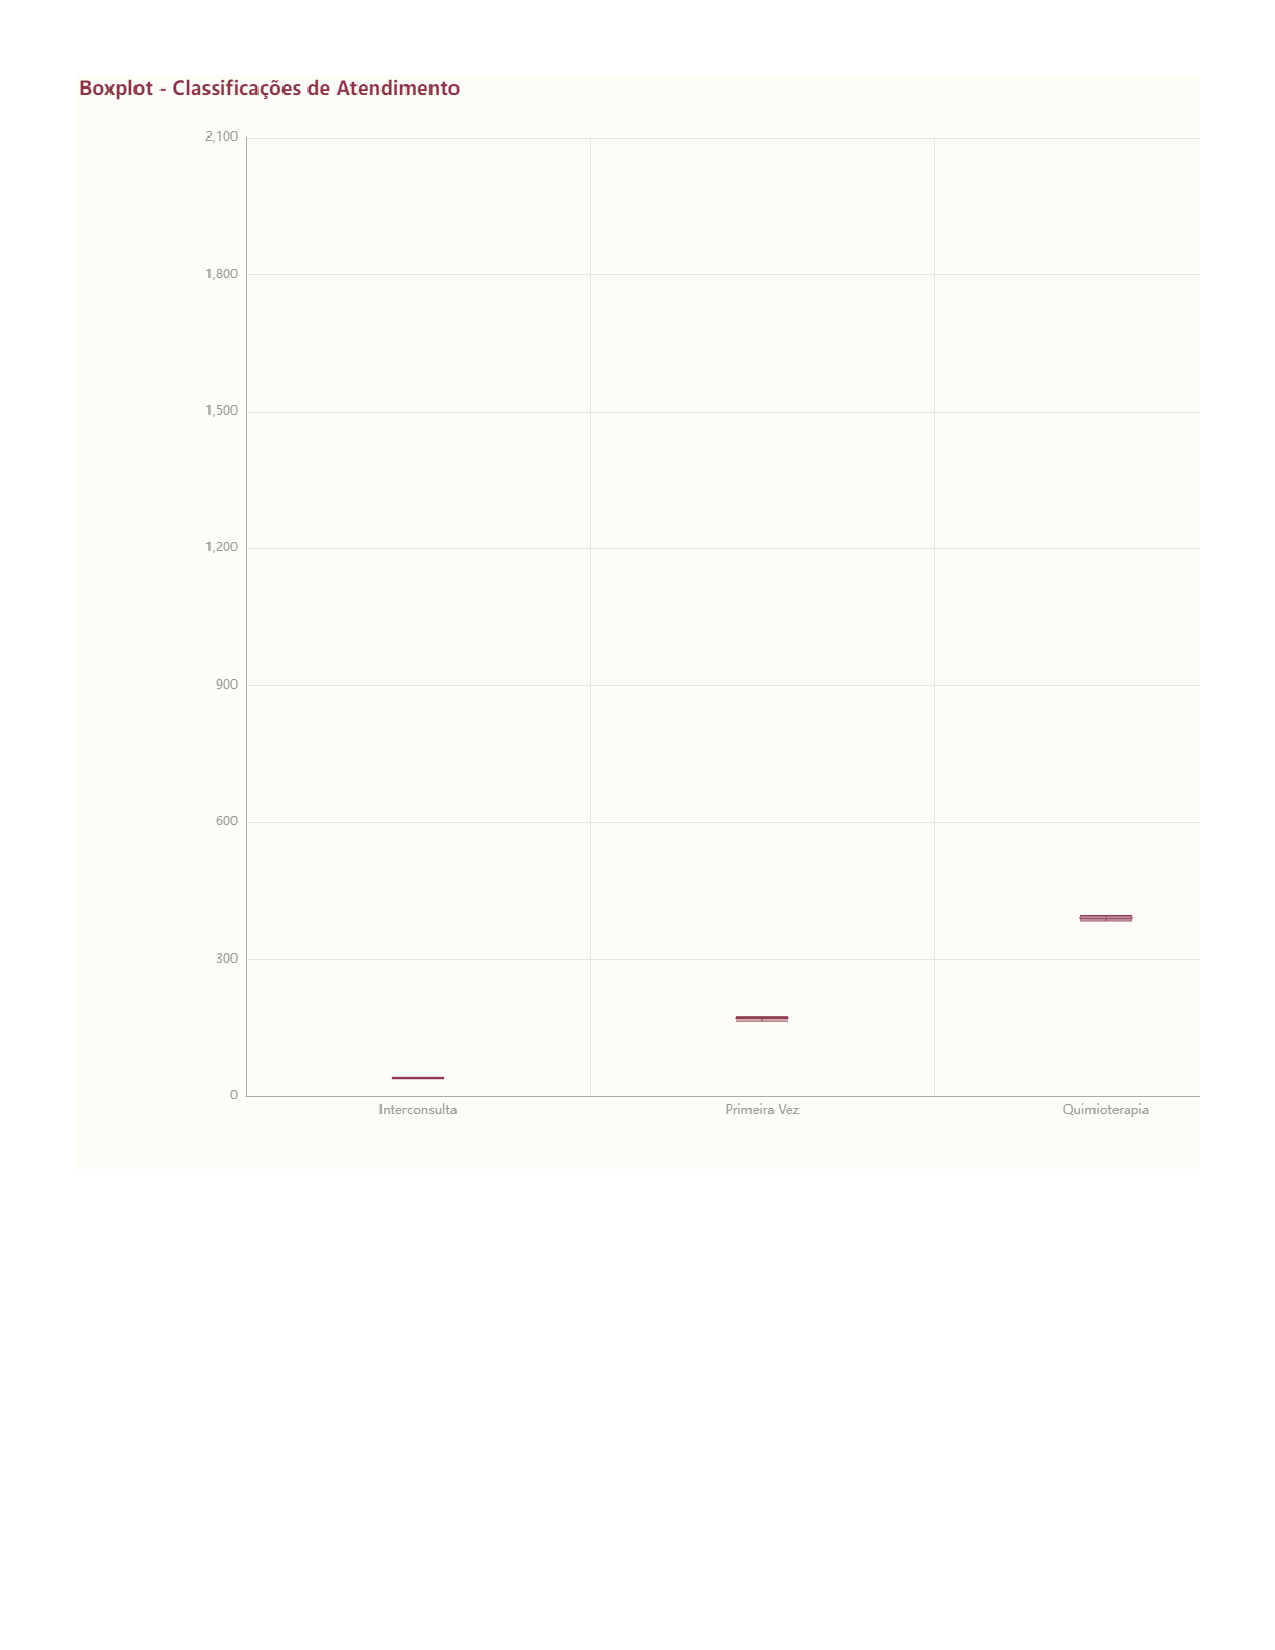
\includegraphics{2023_files/figure-pdf/unnamed-chunk-9-1.pdf}

\part{Parte 04}

\hypertarget{ano-2022-peruxedodo-janeiro---dezembro}{%
\chapter*{Ano: 2022 \textbar{} Período: Janeiro -
Dezembro}\label{ano-2022-peruxedodo-janeiro---dezembro}}
\addcontentsline{toc}{chapter}{Ano: 2022 \textbar{} Período: Janeiro -
Dezembro}

\markboth{Ano: 2022 \textbar{} Período: Janeiro - Dezembro}{Ano: 2022
\textbar{} Período: Janeiro - Dezembro}

\hypertarget{agendamentos-3}{%
\section*{Agendamentos}\label{agendamentos-3}}
\addcontentsline{toc}{section}{Agendamentos}

\markright{Agendamentos}

\section{Parte A}

\begin{table}
\centering
\caption{Tabela 4.1. Frequência absoluta: Agendamentos.}
\centering
\begin{tabular}[t]{>{}c|>{}c}
\hline
Ano & Frequência Absoluta\\
\hline
\textcolor{black}{\em{\textbf{2022}}} & \textcolor{darkblue}{\textbf{26717}}\\
\hline
\multicolumn{2}{l}{\rule{0pt}{1em}\textit{Fonte: } Tasy.}\\
\end{tabular}
\end{table}

\section{Parte B}

\begin{table}
\centering
\caption{Tabela 4.2. Frequências absoluta e relativa: Classificações de Agendamento  <br><i>Valores agrupados por ano e classificações.</i>}
\centering
\begin{tabular}[t]{>{}c|>{}c|>{}c|>{}c}
\hline
Ano & Classificações de Agendamento & Frequência Absoluta & Frequência relativa (em\%)\\
\hline
\textcolor{black}{\em{\textbf{2022}}} & \textcolor{darkgray}{\em{Atendimentos efetuados}} & \textcolor{darkblue}{\textbf{24406}} & \textcolor{darkred}{\textbf{91.4}}\\
\hline
\textcolor{black}{\em{\textbf{2022}}} & \textcolor{darkgray}{\em{Atendimentos não efetuados}} & \textcolor{darkblue}{\textbf{2311}} & \textcolor{darkred}{\textbf{8.6}}\\
\hline
\multicolumn{4}{l}{\rule{0pt}{1em}\textit{Fonte: } Tasy.}\\
\end{tabular}
\end{table}

\section{Parte C}

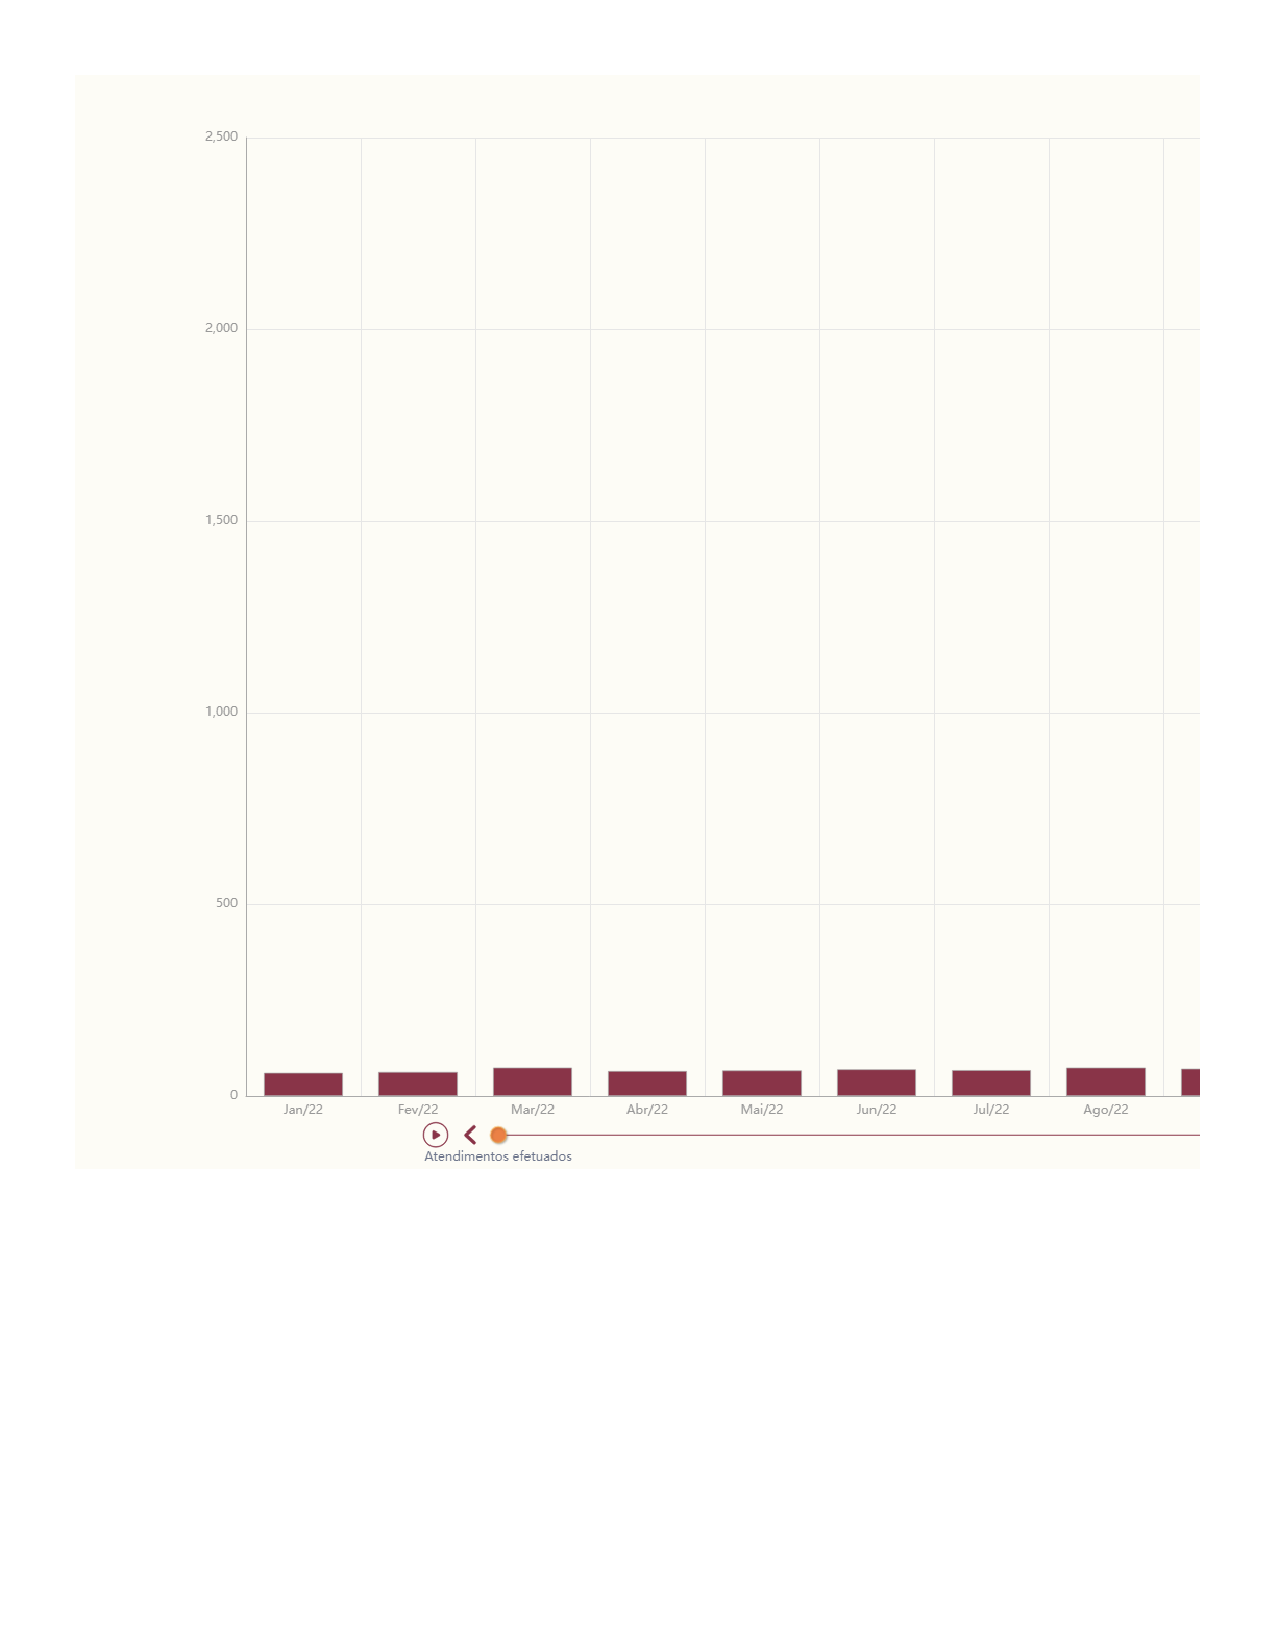
\includegraphics{2022_files/figure-pdf/unnamed-chunk-4-1.pdf}

\section{Parte D}

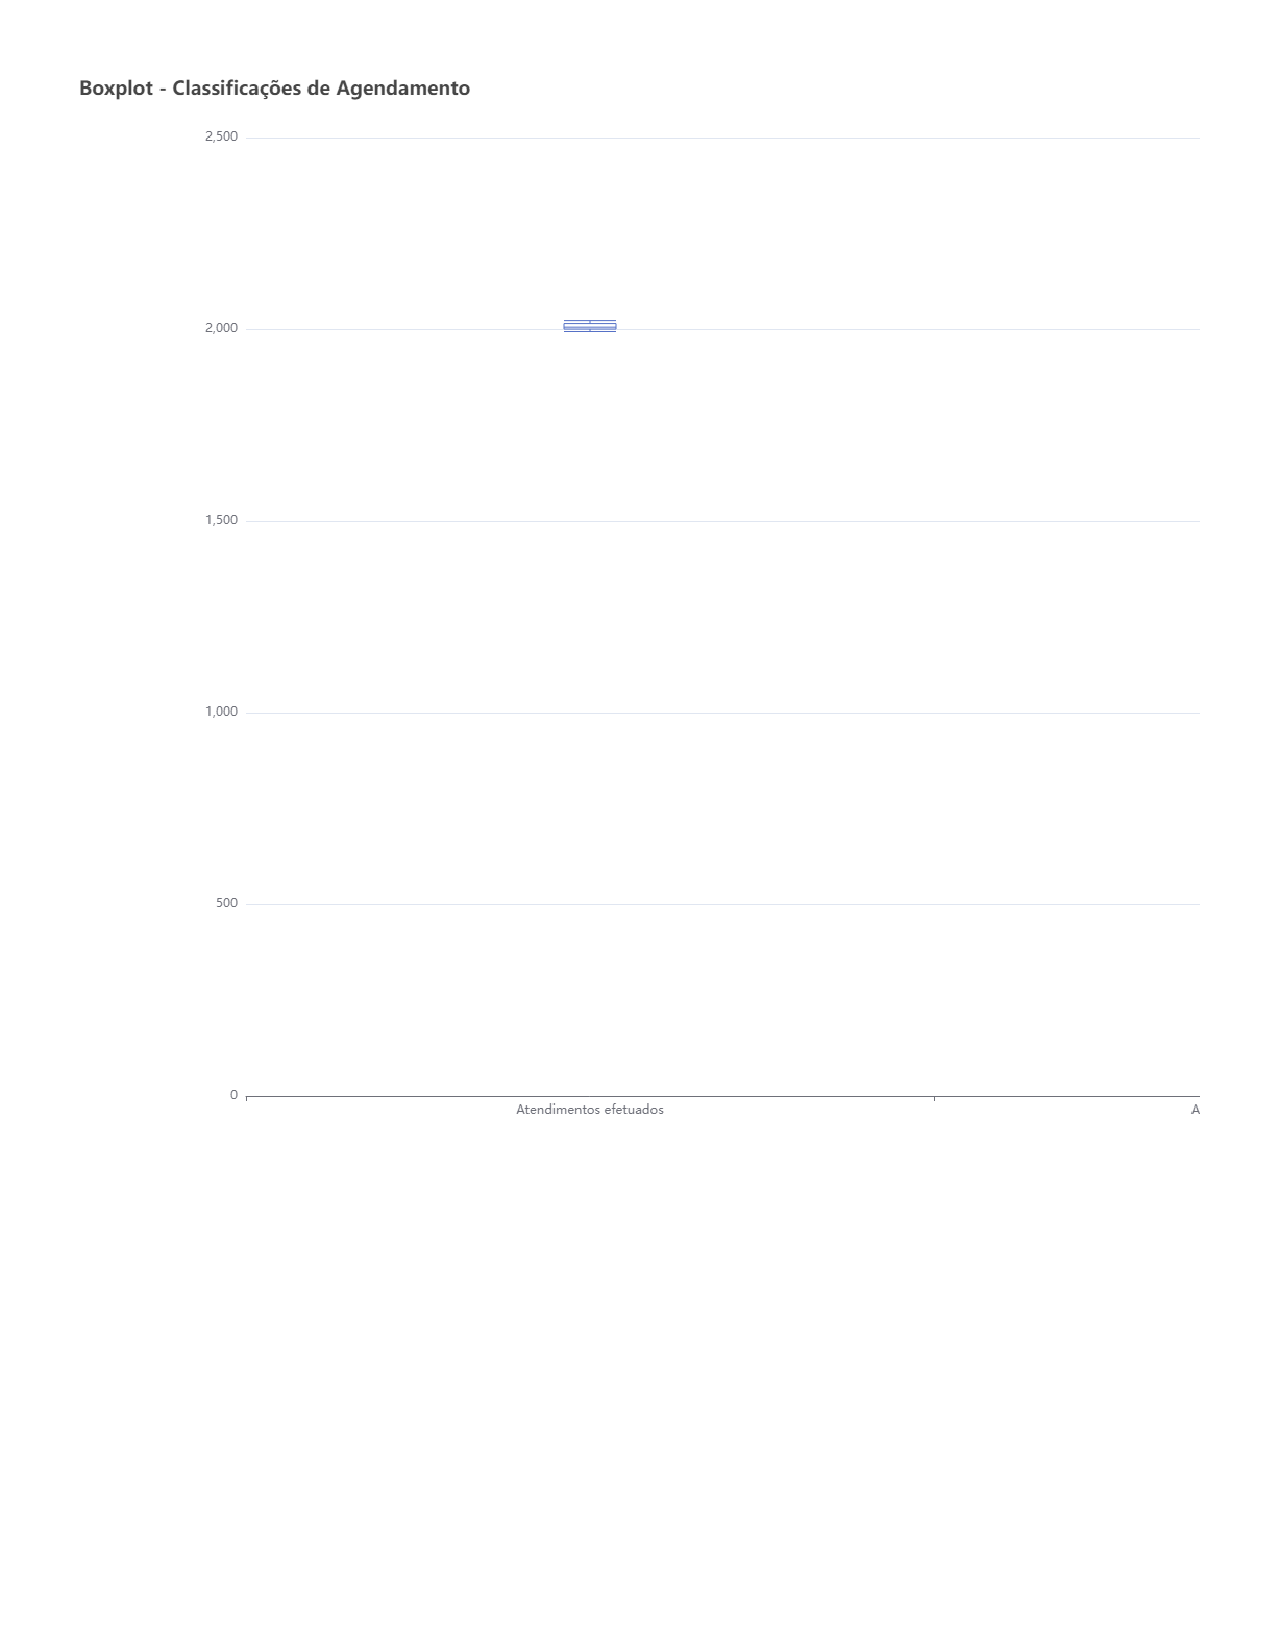
\includegraphics{2022_files/figure-pdf/unnamed-chunk-5-1.pdf}

\hypertarget{atendimentos-3}{%
\section*{Atendimentos}\label{atendimentos-3}}
\addcontentsline{toc}{section}{Atendimentos}

\markright{Atendimentos}

\section{Parte A}

\begin{table}
\centering
\caption{Tabela 2.1. Frequência absoluta: Atendimentos.}
\centering
\begin{tabular}[t]{>{}c|>{}c}
\hline
Ano & Frequência Absoluta\\
\hline
\textcolor{black}{\em{\textbf{2022}}} & \textcolor{darkblue}{\textbf{24406}}\\
\hline
\multicolumn{2}{l}{\rule{0pt}{1em}\textit{Fonte: } Tasy.}\\
\end{tabular}
\end{table}

\section{Parte B}

\begin{table}
\centering
\caption{Tabela 2.2. Frequências absoluta e relativa: Classificações de Agendamento  <br><i>Valores agrupados por ano e classificações.</i>}
\centering
\begin{tabular}[t]{>{}c|>{}c|>{}c|>{}c}
\hline
Ano & Classificações de Atendimento & Frequência Absoluta & Frequência relativa (em\%)\\
\hline
\textcolor{black}{\em{\textbf{2022}}} & \textcolor{darkgray}{\em{Interconsulta}} & \textcolor{darkblue}{\textbf{416}} & \textcolor{darkred}{\textbf{1.7}}\\
\hline
\textcolor{black}{\em{\textbf{2022}}} & \textcolor{darkgray}{\em{Primeira Vez}} & \textcolor{darkblue}{\textbf{2374}} & \textcolor{darkred}{\textbf{9.7}}\\
\hline
\textcolor{black}{\em{\textbf{2022}}} & \textcolor{darkgray}{\em{Quimioterapia}} & \textcolor{darkblue}{\textbf{3283}} & \textcolor{darkred}{\textbf{13.5}}\\
\hline
\textcolor{black}{\em{\textbf{2022}}} & \textcolor{darkgray}{\em{Retorno}} & \textcolor{darkblue}{\textbf{18333}} & \textcolor{darkred}{\textbf{75.1}}\\
\hline
\multicolumn{4}{l}{\rule{0pt}{1em}\textit{Fonte: } Tasy.}\\
\end{tabular}
\end{table}

\section{Parte C}

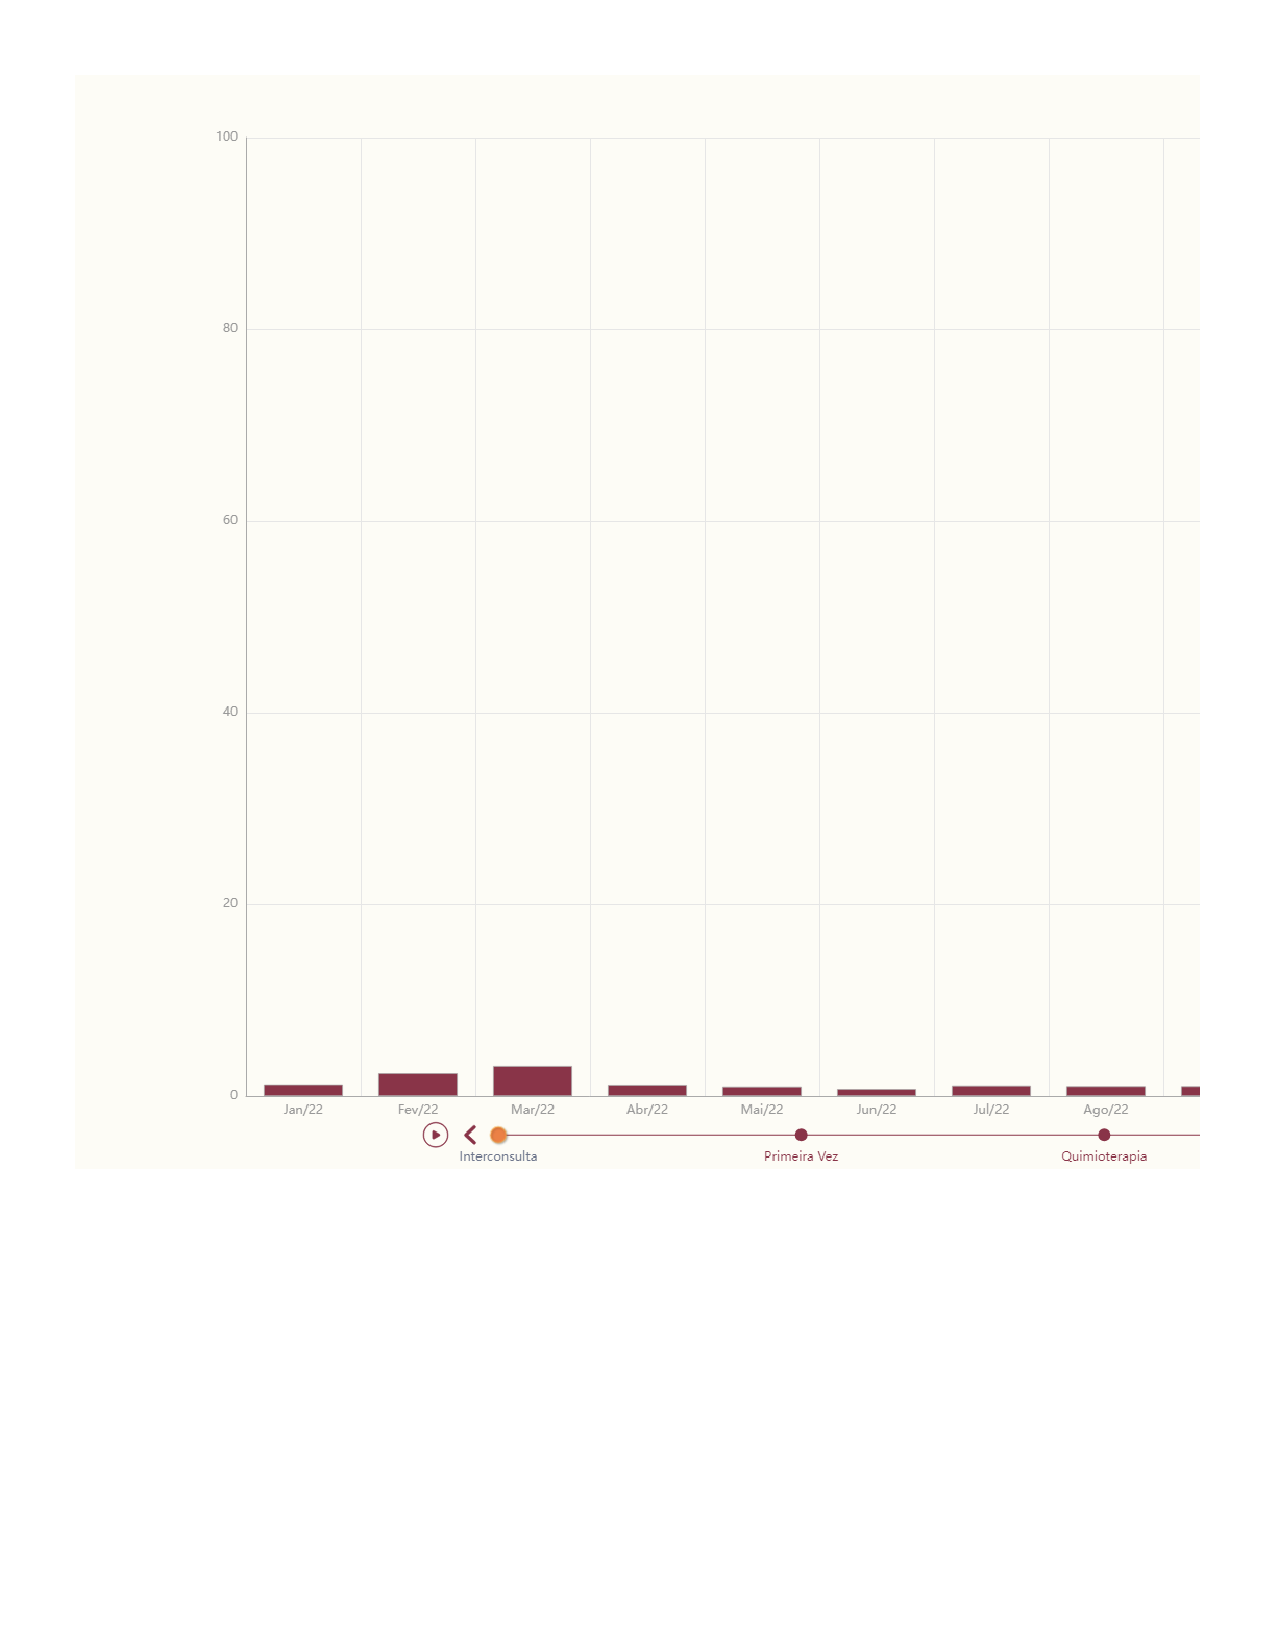
\includegraphics{2022_files/figure-pdf/unnamed-chunk-8-1.pdf}

\section{Parte D}

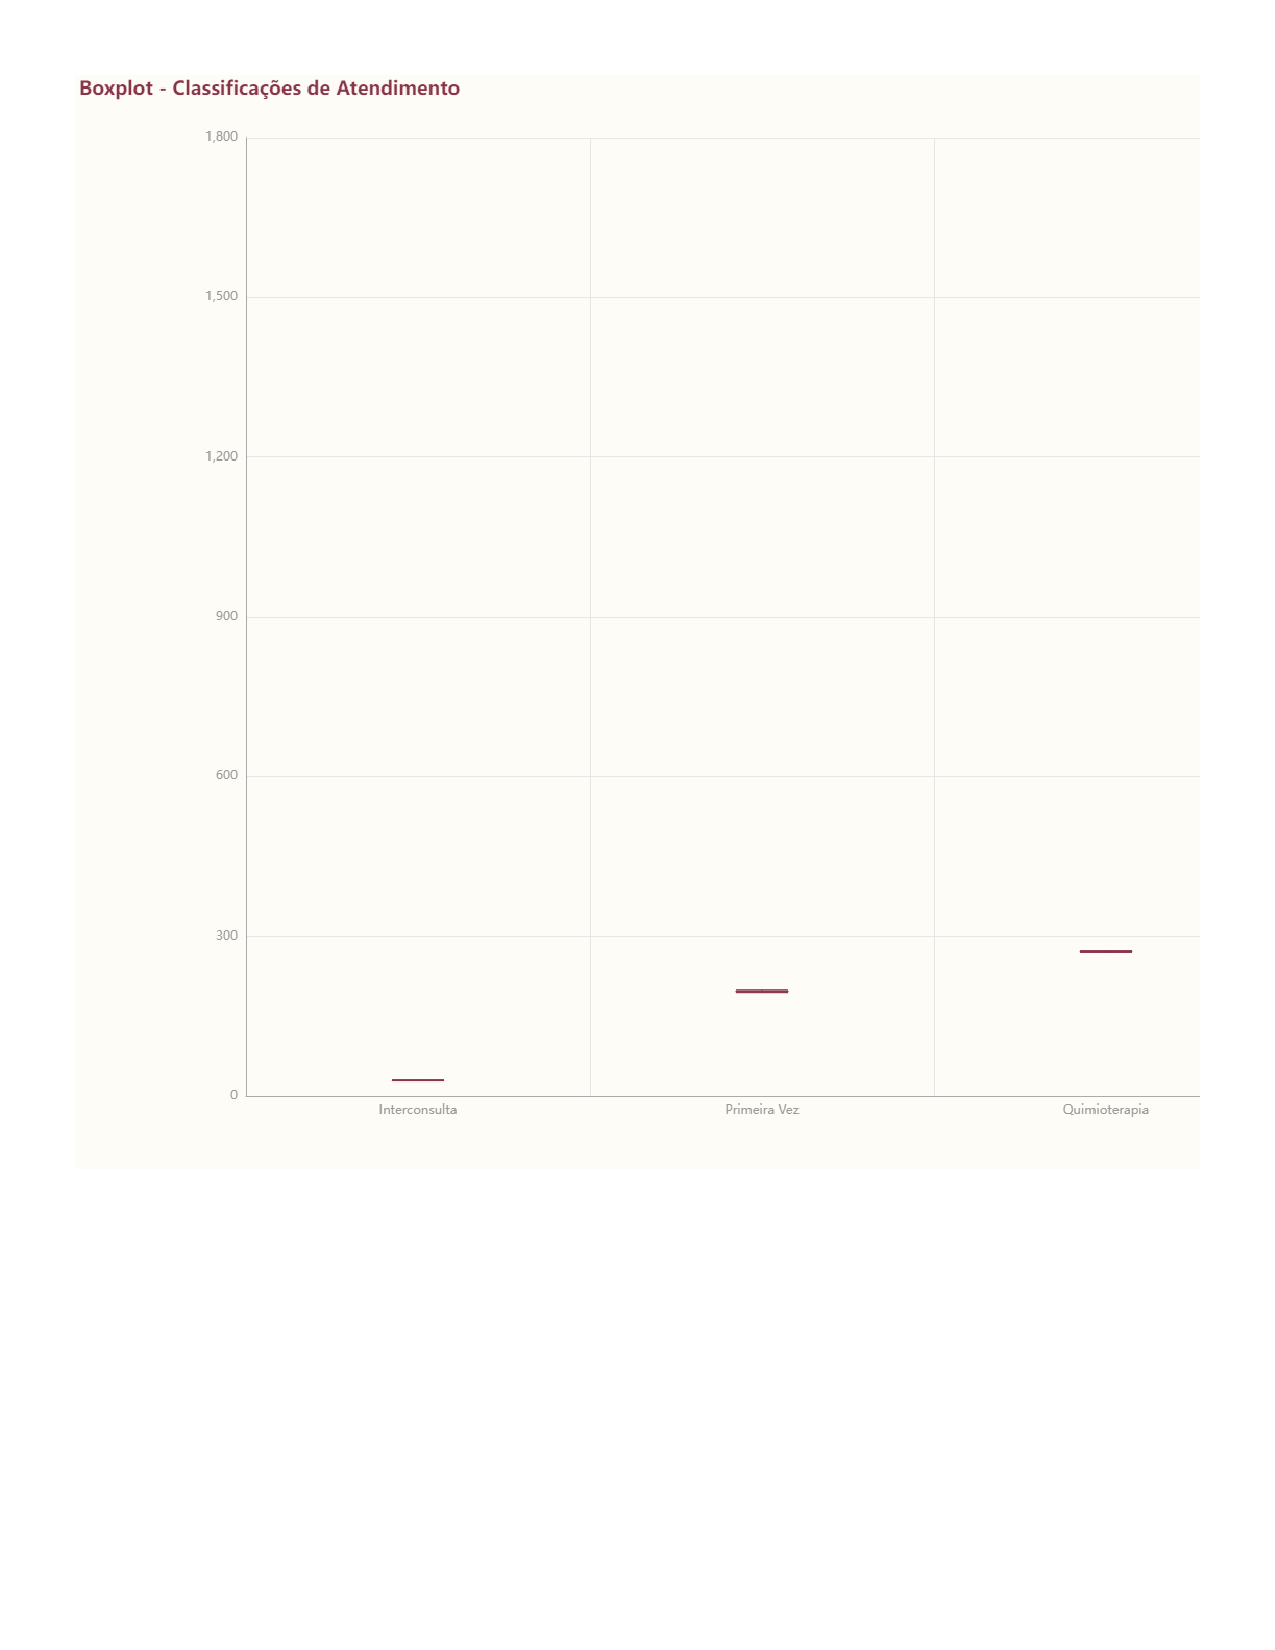
\includegraphics{2022_files/figure-pdf/unnamed-chunk-9-1.pdf}

\part{Parte 05}

\hypertarget{ano-e-peruxedodo-vigentes-1}{%
\chapter*{Ano e Período vigentes}\label{ano-e-peruxedodo-vigentes-1}}
\addcontentsline{toc}{chapter}{Ano e Período vigentes}

\markboth{Ano e Período vigentes}{Ano e Período vigentes}

\hypertarget{agendamentos-4}{%
\section*{Agendamentos}\label{agendamentos-4}}
\addcontentsline{toc}{section}{Agendamentos}

\markright{Agendamentos}

\section{Parte A}

\begin{table}
\centering
\caption{Tabela 1.1. Frequências absoluta e relativa: Agendamentos. <br><i>Valores agrupados por ano.</i>}
\centering
\begin{tabular}[t]{>{}c|>{}c|>{}c}
\hline
Ano & Frequência Absoluta & Frequência relativa (em\%)\\
\hline
\textcolor{black}{\em{\textbf{2022}}} & \textcolor{darkblue}{\textbf{18207}} & \textcolor{darkred}{\textbf{33.2}}\\
\hline
\textcolor{black}{\em{\textbf{2023}}} & \textcolor{darkblue}{\textbf{18736}} & \textcolor{darkred}{\textbf{34.1}}\\
\hline
\textcolor{black}{\em{\textbf{2024}}} & \textcolor{darkblue}{\textbf{17941}} & \textcolor{darkred}{\textbf{32.7}}\\
\hline
\multicolumn{3}{l}{\rule{0pt}{1em}\textit{Fonte: } Tasy.}\\
\end{tabular}
\end{table}

\section{Parte B}

\begin{table}
\centering
\caption{Tabela 1.2. Frequências absoluta e relativa: Classificações de Agendamento  <br><i>Valores agrupados por ano e classificações.</i>}
\centering
\begin{tabular}[t]{>{}c|>{}c|>{}c|>{}c}
\hline
Ano & Classificações de Agendamento & Frequência Absoluta & Frequência relativa (em\%)\\
\hline
\textcolor{black}{\em{\textbf{2022}}} & \textcolor{darkgray}{\em{Atendimentos efetuados}} & \textcolor{darkblue}{\textbf{16461}} & \textcolor{darkred}{\textbf{90.4}}\\
\hline
\textcolor{black}{\em{\textbf{2022}}} & \textcolor{darkgray}{\em{Atendimentos não efetuados}} & \textcolor{darkblue}{\textbf{1746}} & \textcolor{darkred}{\textbf{9.6}}\\
\hline
\textcolor{black}{\em{\textbf{2023}}} & \textcolor{darkgray}{\em{Atendimentos efetuados}} & \textcolor{darkblue}{\textbf{17229}} & \textcolor{darkred}{\textbf{92.0}}\\
\hline
\textcolor{black}{\em{\textbf{2023}}} & \textcolor{darkgray}{\em{Atendimentos não efetuados}} & \textcolor{darkblue}{\textbf{1507}} & \textcolor{darkred}{\textbf{8.0}}\\
\hline
\textcolor{black}{\em{\textbf{2024}}} & \textcolor{darkgray}{\em{Atendimentos efetuados}} & \textcolor{darkblue}{\textbf{17040}} & \textcolor{darkred}{\textbf{95.0}}\\
\hline
\textcolor{black}{\em{\textbf{2024}}} & \textcolor{darkgray}{\em{Atendimentos não efetuados}} & \textcolor{darkblue}{\textbf{901}} & \textcolor{darkred}{\textbf{5.0}}\\
\hline
\multicolumn{4}{l}{\rule{0pt}{1em}\textit{Fonte: } Tasy.}\\
\end{tabular}
\end{table}

\section{Parte C}

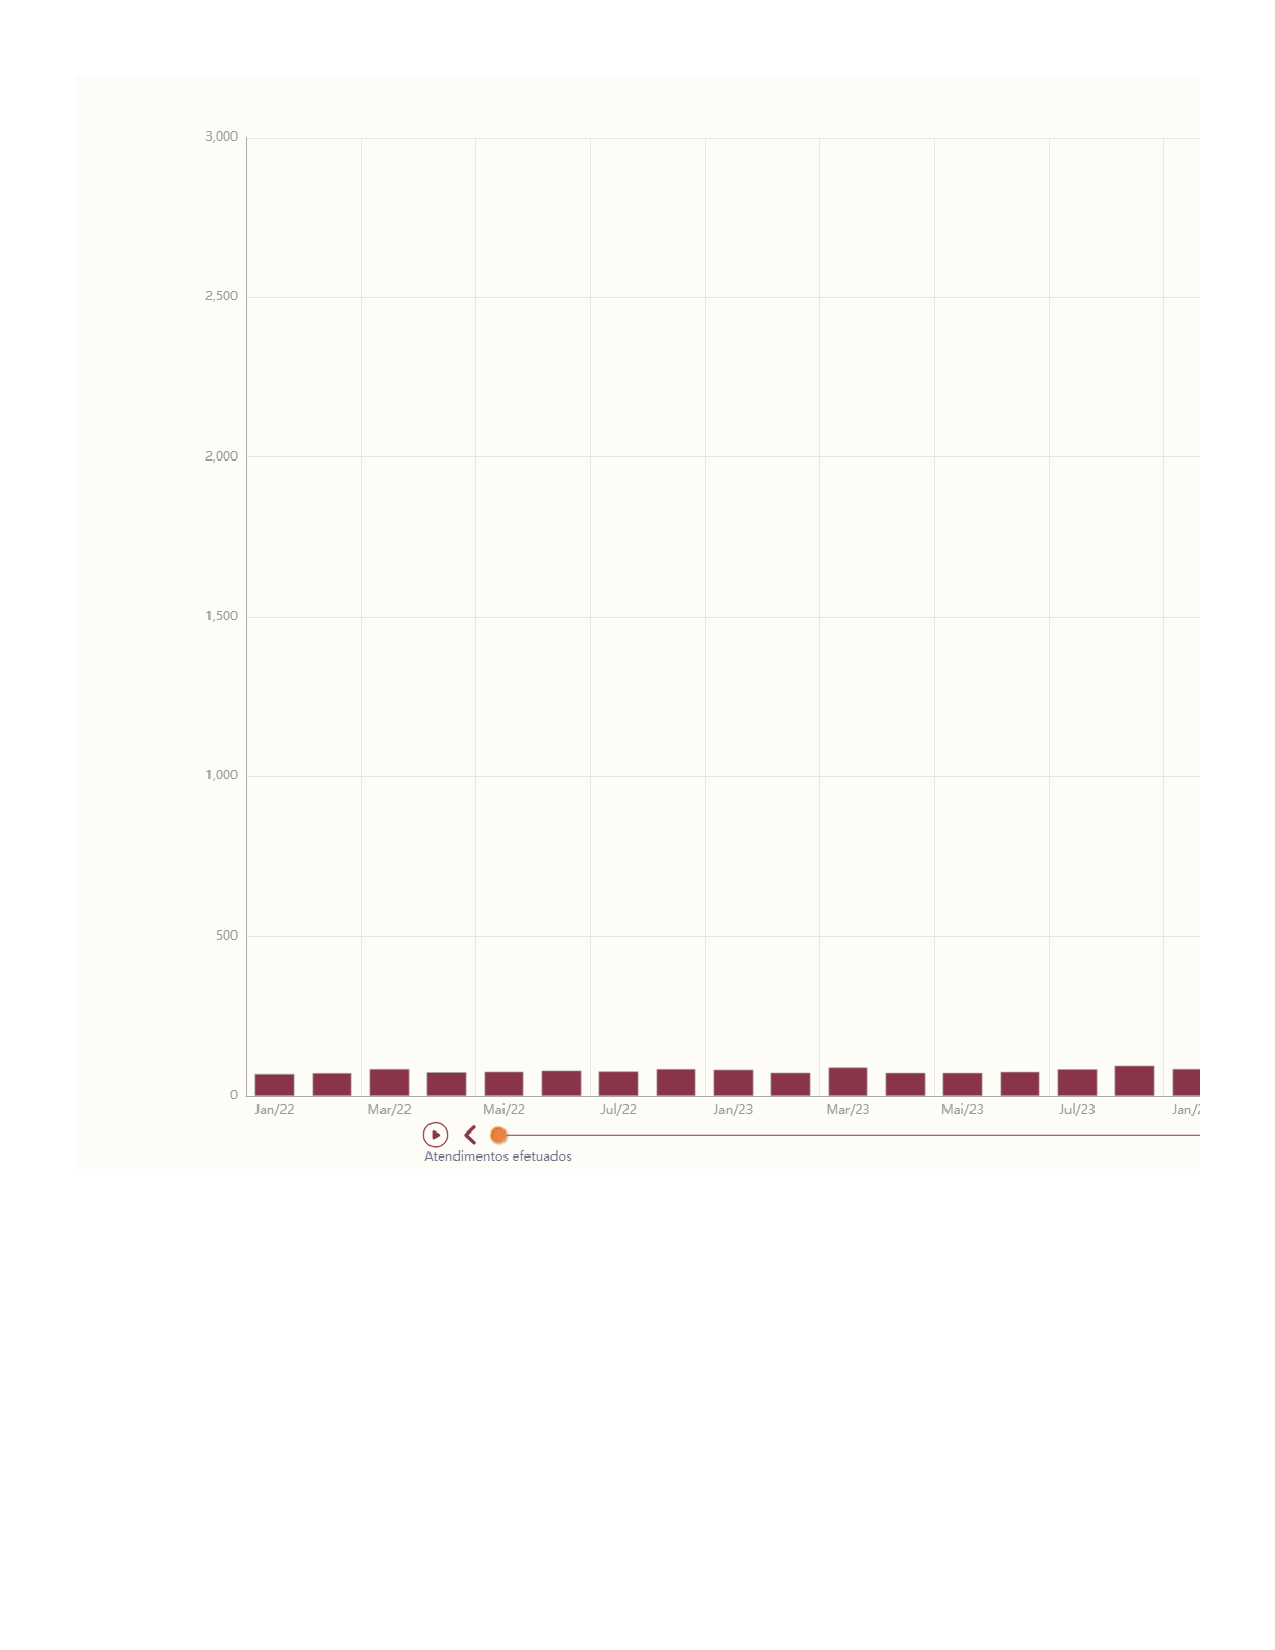
\includegraphics{intro_files/figure-pdf/unnamed-chunk-4-1.pdf}

\section{Parte D}

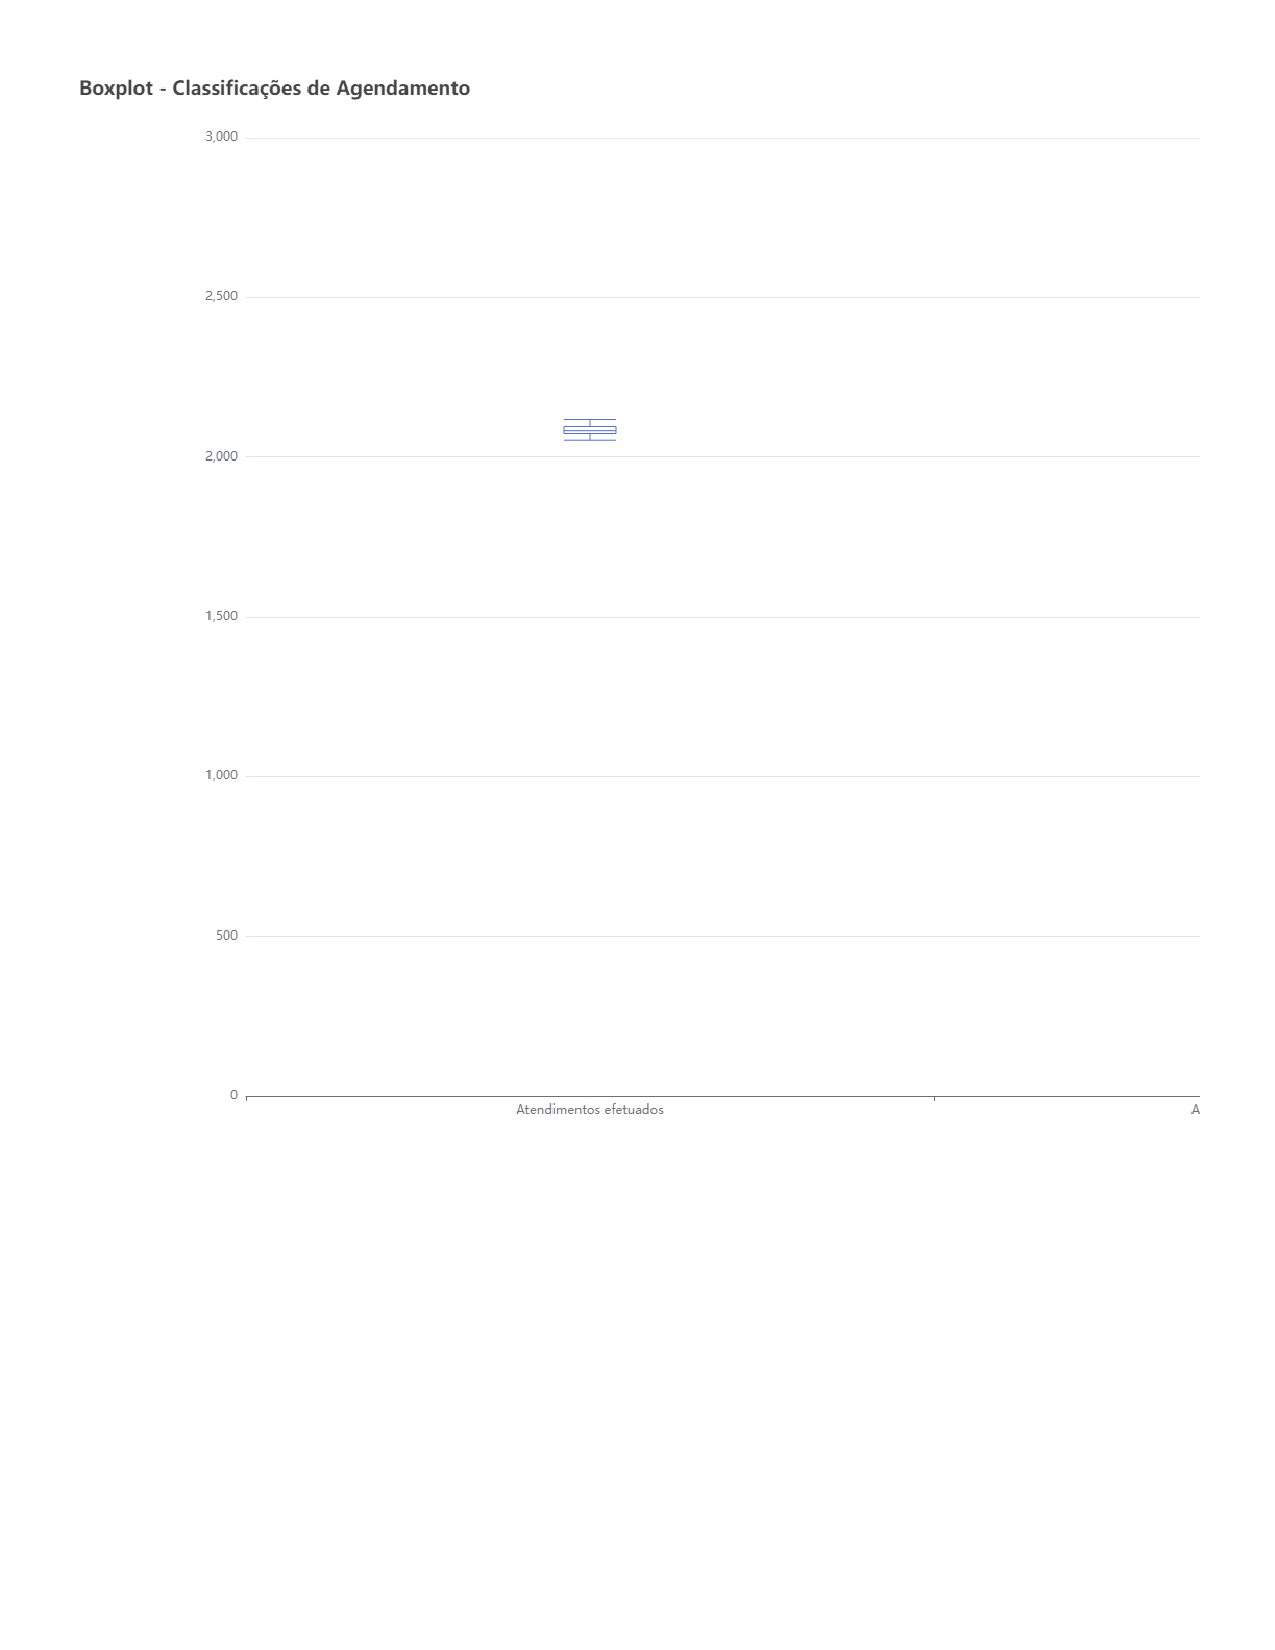
\includegraphics{intro_files/figure-pdf/unnamed-chunk-5-1.pdf}

\hypertarget{atendimentos-4}{%
\section*{Atendimentos}\label{atendimentos-4}}
\addcontentsline{toc}{section}{Atendimentos}

\markright{Atendimentos}

\section{Parte A}

\begin{table}
\centering
\caption{Tabela 2.1. Frequências absoluta e relativa: Agendamentos. <br><i>Valores agrupados por ano.</i>}
\centering
\begin{tabular}[t]{>{}c|>{}c|>{}c}
\hline
Ano & Frequência Absoluta & Frequência relativa (em\%)\\
\hline
\textcolor{black}{\em{\textbf{2022}}} & \textcolor{darkblue}{\textbf{16461}} & \textcolor{darkred}{\textbf{32.4}}\\
\hline
\textcolor{black}{\em{\textbf{2023}}} & \textcolor{darkblue}{\textbf{17229}} & \textcolor{darkred}{\textbf{34.0}}\\
\hline
\textcolor{black}{\em{\textbf{2024}}} & \textcolor{darkblue}{\textbf{17040}} & \textcolor{darkred}{\textbf{33.6}}\\
\hline
\multicolumn{3}{l}{\rule{0pt}{1em}\textit{Fonte: } Tasy.}\\
\end{tabular}
\end{table}

\section{Parte B}

\begin{table}
\centering
\caption{Tabela 2.2. Frequências absoluta e relativa: Classificações de Agendamento  <br><i>Valores agrupados por ano e classificações.</i>}
\centering
\begin{tabular}[t]{>{}c|>{}c|>{}c|>{}c}
\hline
Ano & Classificações de Atendimento & Frequência Absoluta & Frequência relativa (em\%)\\
\hline
\textcolor{black}{\em{\textbf{2022}}} & \textcolor{darkgray}{\em{Interconsulta}} & \textcolor{darkblue}{\textbf{303}} & \textcolor{darkred}{\textbf{1.8}}\\
\hline
\textcolor{black}{\em{\textbf{2022}}} & \textcolor{darkgray}{\em{Primeira Vez}} & \textcolor{darkblue}{\textbf{1577}} & \textcolor{darkred}{\textbf{9.6}}\\
\hline
\textcolor{black}{\em{\textbf{2022}}} & \textcolor{darkgray}{\em{Quimioterapia}} & \textcolor{darkblue}{\textbf{2180}} & \textcolor{darkred}{\textbf{13.2}}\\
\hline
\textcolor{black}{\em{\textbf{2022}}} & \textcolor{darkgray}{\em{Retorno}} & \textcolor{darkblue}{\textbf{12401}} & \textcolor{darkred}{\textbf{75.3}}\\
\hline
\textcolor{black}{\em{\textbf{2023}}} & \textcolor{darkgray}{\em{Interconsulta}} & \textcolor{darkblue}{\textbf{272}} & \textcolor{darkred}{\textbf{1.6}}\\
\hline
\textcolor{black}{\em{\textbf{2023}}} & \textcolor{darkgray}{\em{Primeira Vez}} & \textcolor{darkblue}{\textbf{1551}} & \textcolor{darkred}{\textbf{9.0}}\\
\hline
\textcolor{black}{\em{\textbf{2023}}} & \textcolor{darkgray}{\em{Quimioterapia}} & \textcolor{darkblue}{\textbf{3201}} & \textcolor{darkred}{\textbf{18.6}}\\
\hline
\textcolor{black}{\em{\textbf{2023}}} & \textcolor{darkgray}{\em{Retorno}} & \textcolor{darkblue}{\textbf{12205}} & \textcolor{darkred}{\textbf{70.8}}\\
\hline
\textcolor{black}{\em{\textbf{2024}}} & \textcolor{darkgray}{\em{Interconsulta}} & \textcolor{darkblue}{\textbf{431}} & \textcolor{darkred}{\textbf{2.5}}\\
\hline
\textcolor{black}{\em{\textbf{2024}}} & \textcolor{darkgray}{\em{Primeira Vez}} & \textcolor{darkblue}{\textbf{1457}} & \textcolor{darkred}{\textbf{8.6}}\\
\hline
\textcolor{black}{\em{\textbf{2024}}} & \textcolor{darkgray}{\em{Quimioterapia}} & \textcolor{darkblue}{\textbf{3797}} & \textcolor{darkred}{\textbf{22.3}}\\
\hline
\textcolor{black}{\em{\textbf{2024}}} & \textcolor{darkgray}{\em{Retorno}} & \textcolor{darkblue}{\textbf{11355}} & \textcolor{darkred}{\textbf{66.6}}\\
\hline
\multicolumn{4}{l}{\rule{0pt}{1em}\textit{Fonte: } Tasy.}\\
\end{tabular}
\end{table}

\section{Parte C}

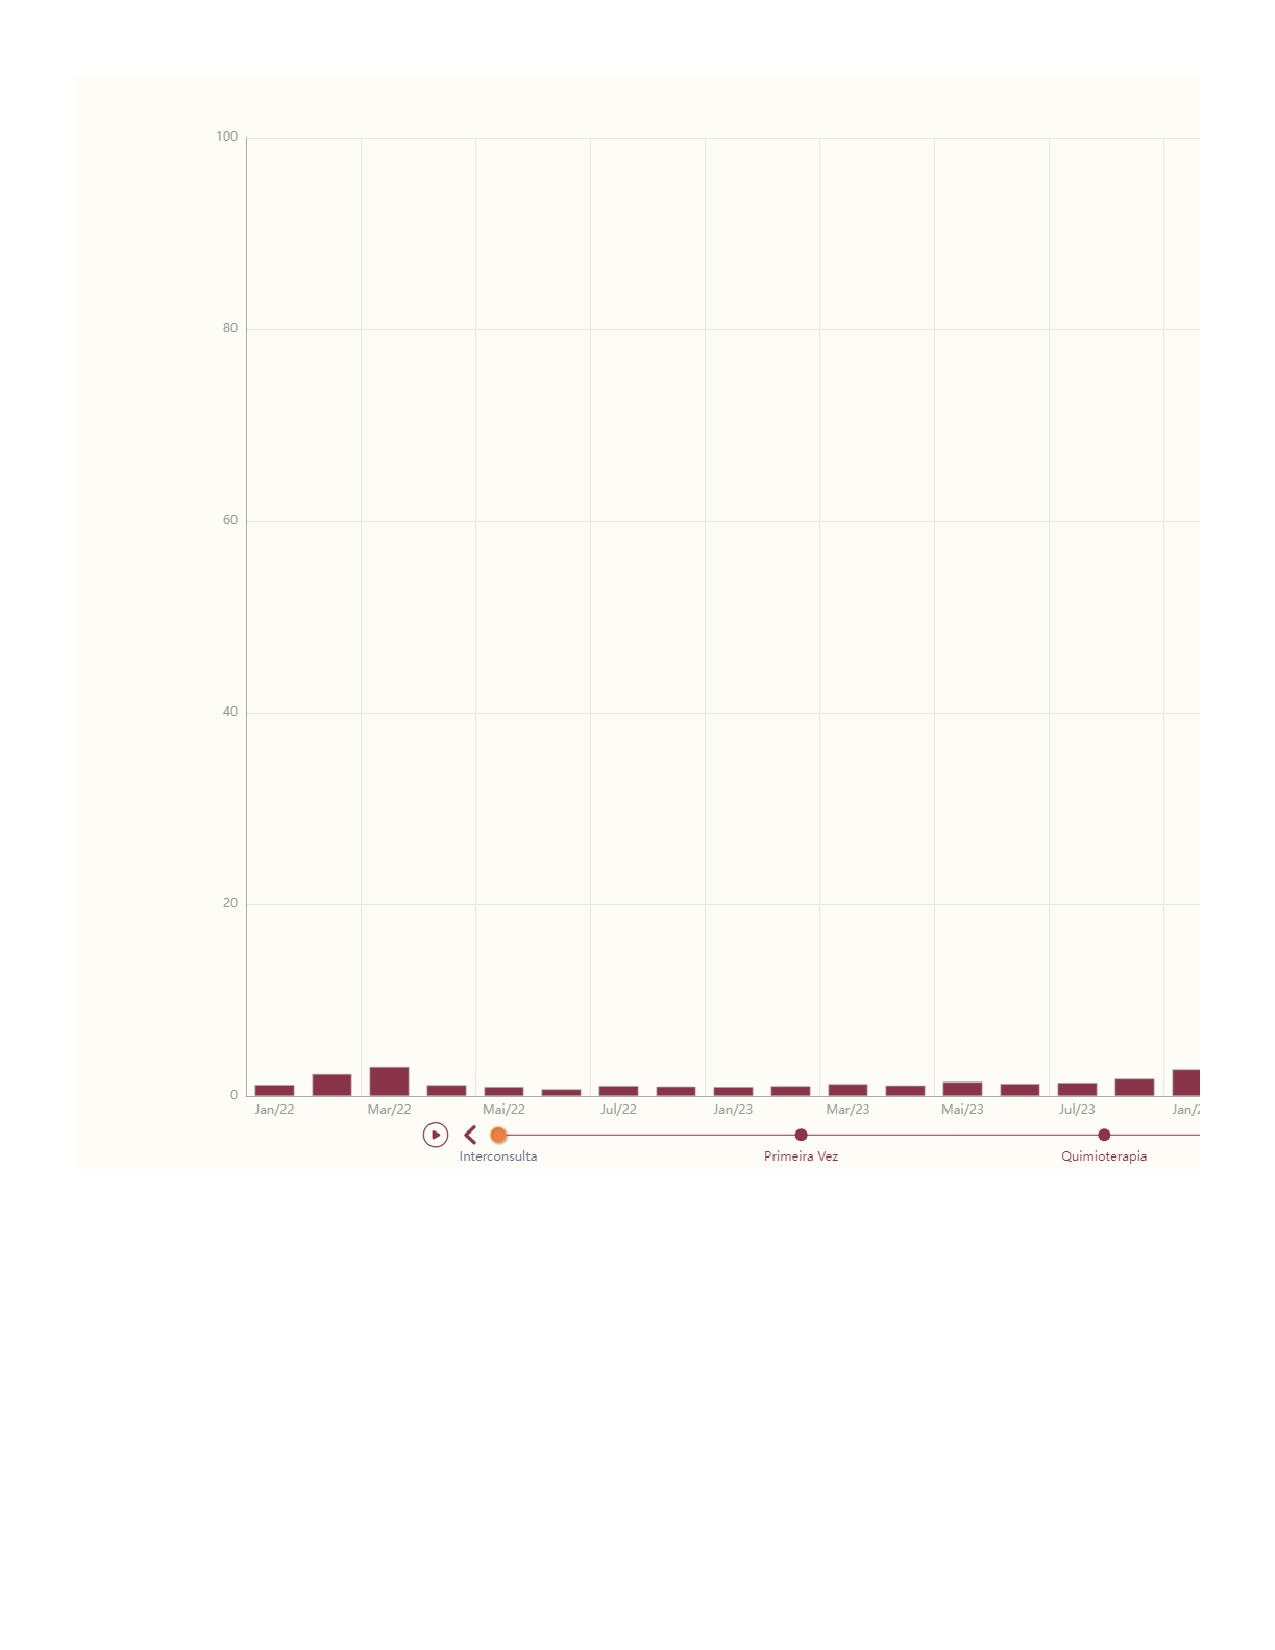
\includegraphics{intro_files/figure-pdf/unnamed-chunk-8-1.pdf}

\section{Parte D}

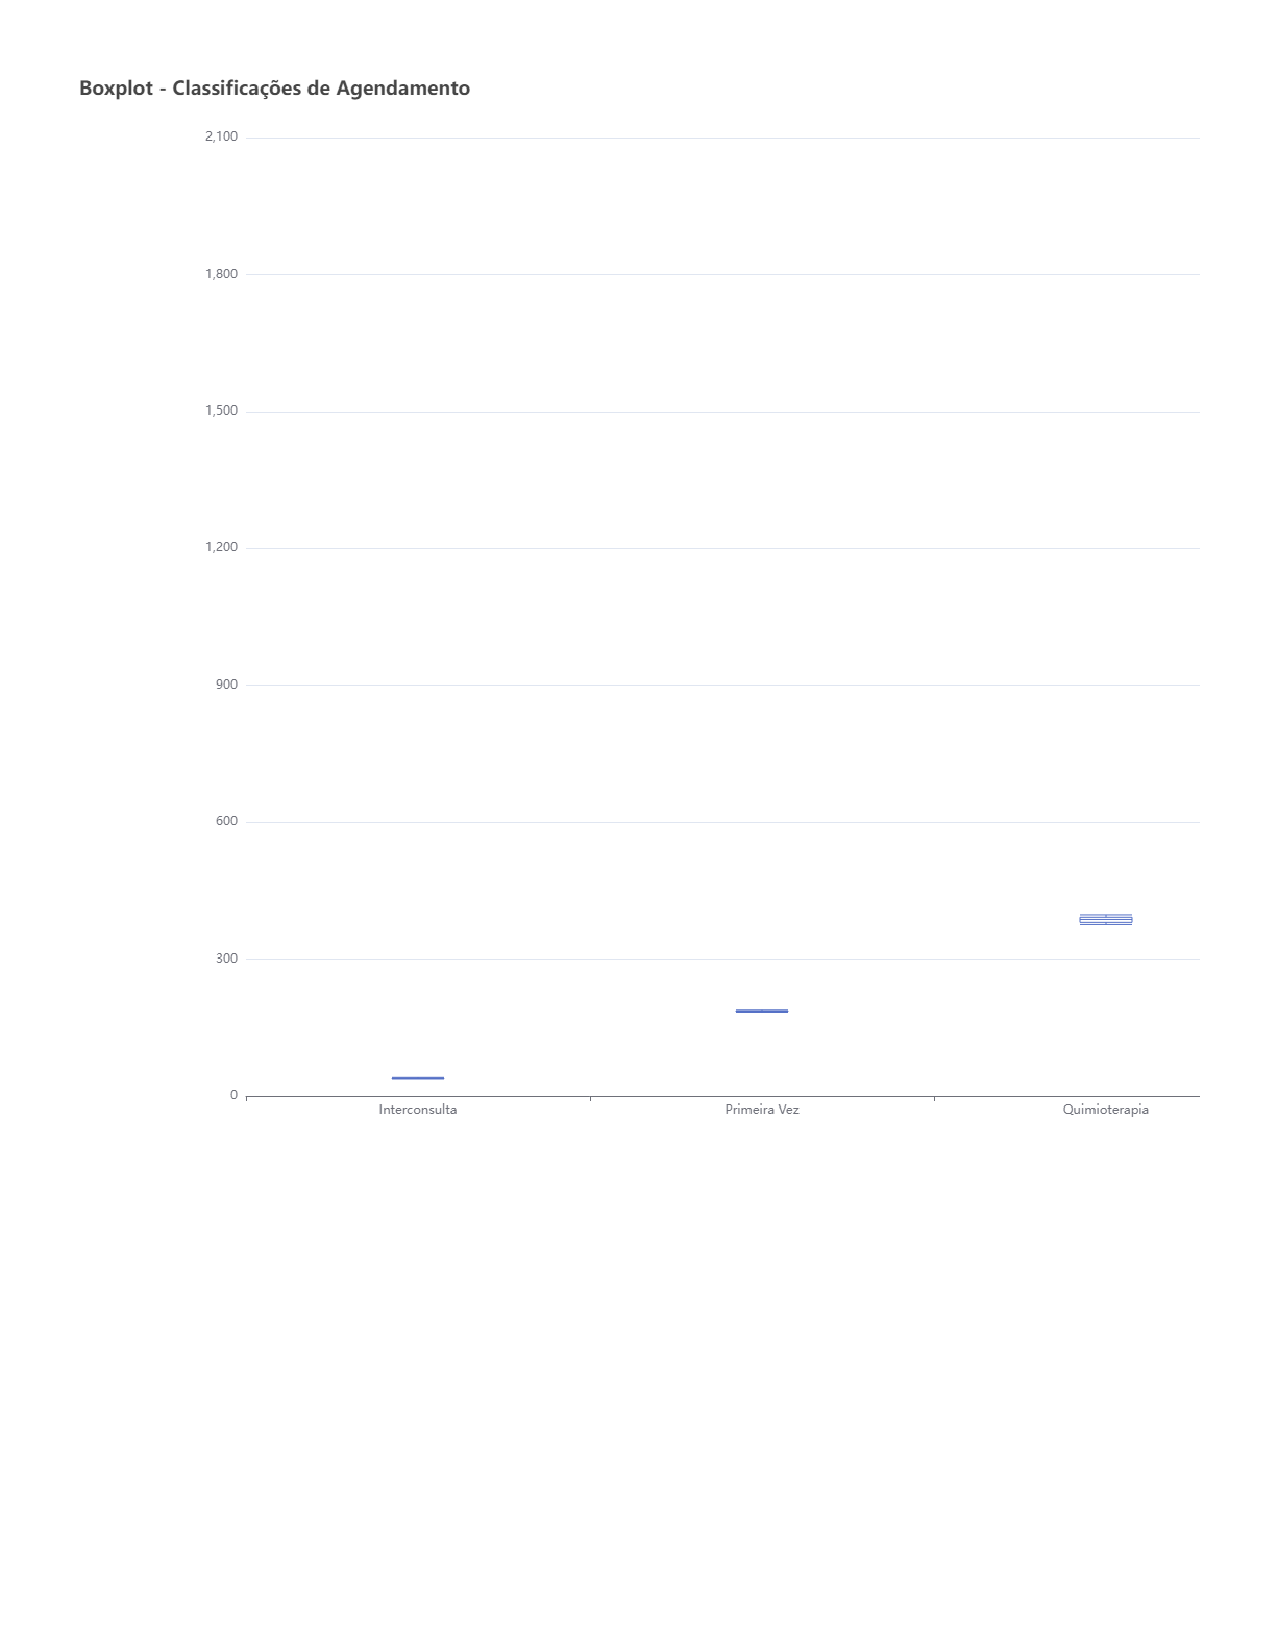
\includegraphics{intro_files/figure-pdf/unnamed-chunk-9-1.pdf}

\bookmarksetup{startatroot}

\hypertarget{references}{%
\chapter*{References}\label{references}}
\addcontentsline{toc}{chapter}{References}

\markboth{References}{References}

\hypertarget{refs}{}
\begin{CSLReferences}{0}{0}
\end{CSLReferences}



\end{document}
